% *** Authors should verify (and, if needed, correct) their LaTeX system  ***
% *** with the testflow diagnostic prior to trusting their LaTeX platform ***
% *** with production work. IEEE's font choices can trigger bugs that do  ***
% *** not appear when using other class files.                            ***
% The testflow support page is at:
% http://www.michaelshell.org/tex/testflow/


%%*************************************************************************
%% Legal Notice:
%% This code is offered as-is without any warranty either expressed or
%% implied; without even the implied warranty of MERCHANTABILITY or
%% FITNESS FOR A PARTICULAR PURPOSE!
%% User assumes all risk.
%% In no event shall IEEE or any contributor to this code be liable for
%% any damages or losses, including, but not limited to, incidental,
%% consequential, or any other damages, resulting from the use or misuse
%% of any information contained here.
%%
%% All comments are the opinions of their respective authors and are not
%% necessarily endorsed by the IEEE.
%%
%% This work is distributed under the LaTeX Project Public License (LPPL)
%% ( http://www.latex-project.org/ ) version 1.3, and may be freely used,
%% distributed and modified. A copy of the LPPL, version 1.3, is included
%% in the base LaTeX documentation of all distributions of LaTeX released
%% 2003/12/01 or later.
%% Retain all contribution notices and credits.
%% ** Modified files should be clearly indicated as such, including  **
%% ** renaming them and changing author support contact information. **
%%
%% File list of work: IEEEtran.cls, New_IEEEtran_how-to.pdf, bare_jrnl_new_sample4.tex,
%%*************************************************************************
\PassOptionsToPackage{unicode}{hyperref}
\PassOptionsToPackage{hyphens}{url}
\PassOptionsToPackage{dvipsnames,svgnames,x11names}{xcolor}
% Note that the a4paper option is mainly intended so that authors in
% countries using A4 can easily print to A4 and see how their papers will
% look in print - the typesetting of the document will not typically be
% affected with changes in paper size (but the bottom and side margins will).
% Use the testflow package mentioned above to verify correct handling of
% both paper sizes by the user's LaTeX system.
%
% Also note that the "draftcls" or "draftclsnofoot", not "draft", option
% should be used if it is desired that the figures are to be displayed in
% draft mode.
%
\documentclass[
  journal,
]{IEEEtran}%
% If IEEEtran.cls has not been installed into the LaTeX system files,
% manually specify the path to it like:
% \documentclass[journal]{../sty/IEEEtran}
\usepackage[cmex10]{amsmath}
\usepackage{amssymb}
\usepackage{iftex}
\ifPDFTeX
  \usepackage[T1]{fontenc}
  \usepackage[utf8]{inputenc}
  \usepackage{textcomp} % provide euro and other symbols
\else % if luatex or xetex
  \usepackage{unicode-math} % this also loads fontspec
  \defaultfontfeatures{Scale=MatchLowercase}
  \defaultfontfeatures[\rmfamily]{Ligatures=TeX,Scale=1}
\fi
%\usepackage{lmodern}
\ifPDFTeX\else
\fi
% Use upquote if available, for straight quotes in verbatim environments
\IfFileExists{upquote.sty}{\usepackage{upquote}}{}
\IfFileExists{microtype.sty}{% use microtype if available
  \usepackage[]{microtype}
  \UseMicrotypeSet[protrusion]{basicmath} % disable protrusion for tt fonts
}{}
\makeatletter
\parindent    1.0em
\ifCLASSOPTIONcompsoc
  \parindent    1.5em
\fi
\makeatother
\usepackage{xcolor}
\setlength{\emergencystretch}{3em} % prevent overfull lines

\setcounter{secnumdepth}{5}
% Make \paragraph and \subparagraph free-standing
\ifx\paragraph\undefined\else
  \let\oldparagraph\paragraph
  \renewcommand{\paragraph}[1]{\oldparagraph{#1}\mbox{}}
\fi
\ifx\subparagraph\undefined\else
  \let\oldsubparagraph\subparagraph
  \renewcommand{\subparagraph}[1]{\oldsubparagraph{#1}\mbox{}}
\fi


\providecommand{\tightlist}{%
  \setlength{\itemsep}{0pt}\setlength{\parskip}{0pt}}\usepackage{longtable,booktabs,array}
\usepackage{calc} % for calculating minipage widths
% Correct order of tables after \paragraph or \subparagraph
\usepackage{etoolbox}
\makeatletter
\patchcmd\longtable{\par}{\if@noskipsec\mbox{}\fi\par}{}{}
\makeatother
% Allow footnotes in longtable head/foot
\IfFileExists{footnotehyper.sty}{\usepackage{footnotehyper}}{\usepackage{footnote}}
\makesavenoteenv{longtable}
\usepackage{graphicx}
\makeatletter
\def\maxwidth{\ifdim\Gin@nat@width>\linewidth\linewidth\else\Gin@nat@width\fi}
\def\maxheight{\ifdim\Gin@nat@height>\textheight\textheight\else\Gin@nat@height\fi}
\makeatother
% Scale images if necessary, so that they will not overflow the page
% margins by default, and it is still possible to overwrite the defaults
% using explicit options in \includegraphics[width, height, ...]{}
\setkeys{Gin}{width=\maxwidth,height=\maxheight,keepaspectratio}
% Set default figure placement to htbp
\makeatletter
\def\fps@figure{htbp}
\makeatother
% definitions for citeproc citations
\NewDocumentCommand\citeproctext{}{}
\NewDocumentCommand\citeproc{mm}{%
  \begingroup\def\citeproctext{#2}\cite{#1}\endgroup}
\makeatletter
 % allow citations to break across lines
 \let\@cite@ofmt\@firstofone
 % avoid brackets around text for \cite:
 \def\@biblabel#1{}
 \def\@cite#1#2{{#1\if@tempswa , #2\fi}}
\makeatother
\newlength{\cslhangindent}
\setlength{\cslhangindent}{1.5em}
\newlength{\csllabelwidth}
\setlength{\csllabelwidth}{3em}
\newenvironment{CSLReferences}[2] % #1 hanging-indent, #2 entry-spacing
 {\begin{list}{}{%
  \setlength{\itemindent}{0pt}
  \setlength{\leftmargin}{0pt}
  \setlength{\parsep}{0pt}
  % turn on hanging indent if param 1 is 1
  \ifodd #1
   \setlength{\leftmargin}{\cslhangindent}
   \setlength{\itemindent}{-1\cslhangindent}
  \fi
  % set entry spacing
  \setlength{\itemsep}{#2\baselineskip}}}
 {\end{list}}
\usepackage{calc}
\newcommand{\CSLBlock}[1]{\hfill\break\parbox[t]{\linewidth}{\strut\ignorespaces#1\strut}}
\newcommand{\CSLLeftMargin}[1]{\parbox[t]{\csllabelwidth}{\strut#1\strut}}
\newcommand{\CSLRightInline}[1]{\parbox[t]{\linewidth - \csllabelwidth}{\strut#1\strut}}
\newcommand{\CSLIndent}[1]{\hspace{\cslhangindent}#1}

\usepackage{booktabs}
\usepackage{longtable}
\usepackage{array}
\usepackage{multirow}
\usepackage{wrapfig}
\usepackage{float}
\usepackage{colortbl}
\usepackage{pdflscape}
\usepackage{tabu}
\usepackage{threeparttable}
\usepackage{threeparttablex}
\usepackage[normalem]{ulem}
\usepackage{makecell}
\usepackage{xcolor}
\usepackage{physics}
\usepackage[version=3]{mhchem}
\usepackage{orcidlink}
\usepackage{float}
\floatplacement{table}{htb}
\usepackage[english]{babel}
\usepackage{bm,bbm}
\usepackage{mathrsfs}
\usepackage{siunitx}
\usepackage{graphicx}
\usepackage{url}
\usepackage[T1]{fontenc}
\usepackage{booktabs}
\usepackage{color}
\usepackage{mathtools}
\usepackage{hyperref}
\usepackage{float}
\usepackage{array}
\usepackage{multirow}
\usepackage{wrapfig}
\usepackage{colortbl}
\usepackage{pdflscape}
\usepackage{xcolor}
\usepackage{amsmath}
\hypersetup{ colorlinks=true, linkcolor=black, filecolor=black, citecolor=black, urlcolor=black}
\makeatletter
\@ifpackageloaded{caption}{}{\usepackage{caption}}
\AtBeginDocument{%
\ifdefined\contentsname
  \renewcommand*\contentsname{Table of contents}
\else
  \newcommand\contentsname{Table of contents}
\fi
\ifdefined\listfigurename
  \renewcommand*\listfigurename{List of Figures}
\else
  \newcommand\listfigurename{List of Figures}
\fi
\ifdefined\listtablename
  \renewcommand*\listtablename{List of Tables}
\else
  \newcommand\listtablename{List of Tables}
\fi
\ifdefined\figurename
  \renewcommand*\figurename{Fig.}
\else
  \newcommand\figurename{Fig.}
\fi
\ifdefined\tablename
  \renewcommand*\tablename{Table}
\else
  \newcommand\tablename{Table}
\fi
}
\@ifpackageloaded{float}{}{\usepackage{float}}
\floatstyle{ruled}
\@ifundefined{c@chapter}{\newfloat{codelisting}{h}{lop}}{\newfloat{codelisting}{h}{lop}[chapter]}
\floatname{codelisting}{Listing}
\newcommand*\listoflistings{\listof{codelisting}{List of Listings}}
\makeatother
\makeatletter
\makeatother
\makeatletter
\@ifpackageloaded{caption}{}{\usepackage{caption}}
\@ifpackageloaded{subcaption}{}{\usepackage{subcaption}}
\makeatother
\usepackage[skip=2pt,font=footnotesize]{caption}
%\captionsetup{format=myformat}
\makeatletter
%\setlength{\cslhangindent}{0pt plus .5pt}
\providecommand{\bibfont}{\footnotesize}
\let\CSLReferences@rig=\CSLReferences
\renewcommand{\CSLReferences}[2]{
\bibfont\settowidth\csllabelwidth{[999]}
\CSLReferences@rig{#1}{#2}
\vskip 0.3\baselineskip plus 0.1\baselineskip minus 0.1\baselineskip%
}
\makeatother
\ifLuaTeX
  \usepackage{selnolig}  % disable illegal ligatures
\fi
\IfFileExists{bookmark.sty}{\usepackage{bookmark}}{\usepackage{hyperref}}
\IfFileExists{xurl.sty}{\usepackage{xurl}}{} % add URL line breaks if available
\urlstyle{same} % disable monospaced font for URLs
\hypersetup{
  pdftitle={Rényi Entropy-Based Heterogeneity Detection in SAR Data},
  pdfauthor={Janeth Alpala, Abraão D.~C.~Nascimento; Alejandro C.~Frery},
  pdfkeywords={Rényi entropy, Gamma
distribution, heterogeneity, SAR, hypothesis tests},
  colorlinks=true,
  linkcolor={black},
  filecolor={Maroon},
  citecolor={black},
  urlcolor={black},
  pdfcreator={LaTeX via pandoc}}

% *** Do not adjust lengths that control margins, column widths, etc. ***
% *** Do not use packages that alter fonts (such as pslatex).         ***
% There should be no need to do such things with IEEEtran.cls V1.6 and later.
% (Unless specifically asked to do so by the journal or conference you plan
% to submit to, of course. )


% correct bad hyphenation here
\hyphenation{op-tical net-works semi-conduc-tor}

%
% paper title
% can use linebreaks \\ within to get better formatting as desired
% Do not put math or special symbols in the title.
% paper title
% can use linebreaks \\ within to get better formatting as desired
% Do not put math or special symbols in the title.
\title{Rényi Entropy-Based Heterogeneity Detection in SAR Data}

\author{
Janeth Alpala, Abraão D.~C.~Nascimento
and~Alejandro C.~Frery%
\thanks{Janeth Alpala, Abraão D.~C.~Nascimento is with Departamento de
Estatística, Universidade Federal de Pernambuco, Recife, 50670-901 PE,
Brazil%
 e-mail: janeth.alpala@ufpe.br, abraao@de.ufpe.br}
%by-author.affiliations
\thanks{Alejandro C.~Frery is with School of Mathematics and
Statistics, Victoria University of Wellington, Wellington, 6140 New
Zealand%
 e-mail: alejandro.frery@vuw.ac.nz}
%by-author.affiliations
}
\begin{document}

% The paper headers
\markboth{Journal XXX, Month Year}{}

% use for special paper notices

% make the title area
\maketitle

% As a general rule, do not put math, special symbols or citations
% in the abstract or keywords.
\begin{abstract}
Synthetic aperture radar (SAR) systems have already been successfully
used to solve remote sensing problems. A disadvantage of SAR images is
the presence of speckle, which is fully developed in homogeneous areas
and gamma-distributed in these scenes. In heterogeneous areas, the
intensity values are \(\mathcal{G}^0_I\)-distributed. In this way, the
identification of roughness SAR areas (as opposed to homogeneous ones)
is an important task. In this work, we propose a family of hypothesis
tests driven by an order parameter to identify roughness features in SAR
intensity data using Rényi entropy. In particular, we use a
nonparametric estimator for the Rényi entropy and investigate some of
its properties. As a practical evaluation method, we develop \(p\)-value
maps on which one can observe both (i) the heterogeneous evidence change
per texture and (ii) the prediction of homogeneous and heterogeneous
categories. The results are in favor of the Rényi-based heterogeneity
detector compared to the one based on Shannon entropy.
\end{abstract}
% Note that keywords are not normally used for peerreview papers.
\begin{IEEEkeywords}
Rényi entropy, Gamma distribution, heterogeneity, SAR, hypothesis tests
\end{IEEEkeywords}

% For peer review papers, you can put extra information on the cover
% page as needed:
% \ifCLASSOPTIONpeerreview
% \begin{center} \bfseries EDICS Category: 3-BBND \end{center}
% \fi
%
% For peerreview papers, this IEEEtran command inserts a page break and
% creates the second title. It will be ignored for other modes.
% \IEEEpeerreviewmaketitle


\section{Introduction}\label{introduction}

\IEEEPARstart{S}{ynthetic} Aperture Radar (SAR) technology has become
essential for a wide range of
applications~\citeproc{ref-Yu2023}{{[}1{]}}--\citeproc{ref-Mondini2021}{{[}3{]}}.
It provides high-resolution data that is independent of sunlight and
operates in a variety of weather conditions to facilitate global Earth
monitoring~\citeproc{ref-Zeng2020}{{[}4{]}}. Despite its advantages, the
effective use of SAR data depends on understanding its statistical
properties because this data is affected by speckle, a noise-like
interference effect~\citeproc{ref-Argenti2013}{{[}5{]}},
\citeproc{ref-Choi2019}{{[}6{]}}. In intensity format, speckle is
typically non-Gaussian, and its presence complicates subsequent image
analysis tasks.

The \(\mathcal{G}^0_I\) distribution has been shown to be an effective
law for SAR intensity data, as it captures different levels of
roughness. A special case is the Gamma distribution, which arises when
speckle is fully developed, indicating homogeneous regions. Although
these assumptions offer flexibility in describing SAR intensities,
selecting the appropriate distribution can be challenging for two main
reasons: the small sample sizes used in practical applications and the
inherent difficulties associated with parameter estimation. These
challenges complicate model selection and highlight the need to explore
alternative statistical approaches.

Entropy measures have gained attention as valuable statistical tools for
analyzing SAR data, with applications in edge
detection~\citeproc{ref-Nascimento2014}{{[}7{]}},
segmentation~\citeproc{ref-Nobre2016}{{[}8{]}},
classification~\citeproc{ref-Cassetti2022}{{[}9{]}}, and noise
reduction~\citeproc{ref-Chan2022}{{[}10{]}}. Traditionally, Shannon
entropy~\citeproc{ref-Shannon1948}{{[}11{]}} has been widely used to
quantify uncertainty and disorder in data. However, this study explores
an alternative information measure: Rényi entropy---a generalization of
Shannon's formulation. This more flexible approach provides additional
insights for identifying heterogeneity, making it a promising tool for
enhancing SAR image analysis.

In this work, we propose a statistical test based on a non-parametric
estimator of Rényi entropy to identify heterogeneous regions in SAR
data. The test assesses whether the observed Rényi entropy in a given
region significantly differs from its expected theoretical value under
the assumption of homogeneity. Compared to our previous approach using
Shannon entropy~\citeproc{ref-Frery2024}{{[}12{]}}, the Rényi-based
approach improves the detection of heterogeneity in real SAR images.

The remainder of this article is organized as follows.
Section~\ref{sec:pre} outlines an overview of statistical models for SAR
intensity data and introduces Rényi entropy. Section~\ref{sec:met}
describes the proposed hypothesis test and the formulation of the test
statistic. Section~\ref{sec:app} evaluates the performance of the test
using real SAR data. Finally, the concluding remarks are drawn in
Section~\ref{sec:conclusion}.

\section{PRELIMINARIES}\label{sec:pre}

\subsection{Statistical Models}\label{statistical-models}

The main distributions considered for SAR intensity data are the
\(\Gamma_{\text{SAR}}\) distribution, which is suitable for fully
developed speckle, and the \(\mathcal{G}^0_I\) distribution, which is
able to describe roughness~\citeproc{ref-Frery1997}{{[}13{]}}. These
distributions are characterized by the following probability density
functions (pdfs): \begin{align}
    f_{\Gamma_{\text{SAR}}}\bigl(z;L, \mu \bigr) 
    &= \frac{L^L}{\Gamma(L)\,\mu^L} z^{L-1} 
    \exp \biggl(-\frac{Lz}{\mu}\biggr)
    \mathbbm 1_{\mathbbm R_+}(z) \label{E:gamma1}
    \intertext{and}
    f_{\mathcal{G}^0_I}\bigl(z; \mu, \alpha, L \bigr) 
    &= \frac{L^L\,\Gamma(L-\alpha)}
    {\bigl[-\mu(\alpha+1)\bigr]^{\alpha} \Gamma(-\alpha)\,\Gamma(L)}
    \notag \\
    &\quad \times
    \frac{z^{L-1}}
    {\bigl[-\mu(\alpha+1)+Lz\bigr]^{L-\alpha}}
    \mathbbm 1_{\mathbbm R_+}(z), \label{E:gi01}
\end{align} where \(\mu > 0\) is the mean, \(\alpha < 0\) measures the
roughness, \(L \geq 1\) is the number of looks, \(\Gamma(\cdot)\) is the
gamma function, and \(\mathbbm 1_{A}(z)\) is the indicator function of
the set \(A\). As demonstrated by~\citeproc{ref-Frery1997}{{[}13{]}},
the \(\Gamma_{\text{SAR}}\) model is a particular case of the
\(\mathcal{G}^0_I\) distribution. Specifically, for a given \(\mu\)
fixed, \[
f_{\mathcal{G}^0_I}\big(z; \mu, \alpha, L\big)
\longrightarrow 
f_{\Gamma_{\text{SAR}}}(z;L, \mu) 
\] when \(\alpha\to-\infty\).

\subsection{Rényi Entropy}\label{ruxe9nyi-entropy}

Introduced by Alfréd Rényi in
1961~\citeproc{ref-renyi1961measures}{{[}14{]}}, this measure
generalizes several well-known entropies, including the Shannon
entropy~\citeproc{ref-Ribeiro2021}{{[}15{]}}. For a continuous random
variable \(Z\) with pdf \(f(z)\), the Rényi entropy of order
\(\lambda\), with \(\lambda > 0\) and \(\lambda \neq 1\), is defined as:
\begin{equation}
\label{E:entropy2}
H_\lambda(Z) = \frac{1}{1 - \lambda} \ln \int_{-\infty}^{\infty} [f(z)]^\lambda \, dz.
\end{equation} Using \eqref{E:entropy2}, we derive closed-form
expressions for the Rényi entropy of the \(\Gamma_{\mathrm{SAR}}\) and
\(\mathcal{G}^0_I\) distributions: \begin{multline}
\label{eq-HGammaSAR}
H_\lambda\bigl(\Gamma_{\text{SAR}}(L, \mu)\bigr)
= 
\ln \mu - \ln L + \frac{1}{1-\lambda}
\Bigl[
  -\lambda\,\ln\Gamma(L) \\  + \ln\Gamma\bigl(\lambda(L-1)+1\bigr)  - \bigl(\lambda(L-1)+1\bigr)\,\ln\lambda
\Bigr]
\end{multline} and \begin{multline}\label{eq-HGI0}
H_\lambda\bigl(\mathcal{G}^0_I(\mu, \alpha, L)\bigr)=\ln\mu-\ln L +\ln(-1 - \alpha)\\
+ \frac{1}{\,1 - \lambda\,}
\Bigl[
   \lambda\bigl(
      \ln\Gamma(L - \alpha)
      -\ln\Gamma(-\alpha)
      -\ln\Gamma(L)
   \bigr)\\
   +\ln\Gamma\bigl(\lambda(L - 1) + 1\bigr)
   +\ln\Gamma\bigl(\lambda(-\alpha + 1) - 1\bigr)\\
   -\ln\Gamma\bigl(\lambda(L - \alpha)\bigr)
\Bigr].
\end{multline} The derivation of this result is given in the Appendix.

Fig.~\ref{fig-plot} presents the Rényi entropy of \(\mathcal{G}^0_I\) as
a function of \(\mu\) for different \(\alpha\) values. As
\(\alpha \to -\infty\), it approaches the Rényi entropy of
\(\Gamma_{\text{SAR}}\), which is aligned with the fact that
\(\Gamma_{\text{SAR}}\) is a limiting case of the \(\mathcal{G}^0_I\)
model.

\begin{figure}[hbt]

\centering{

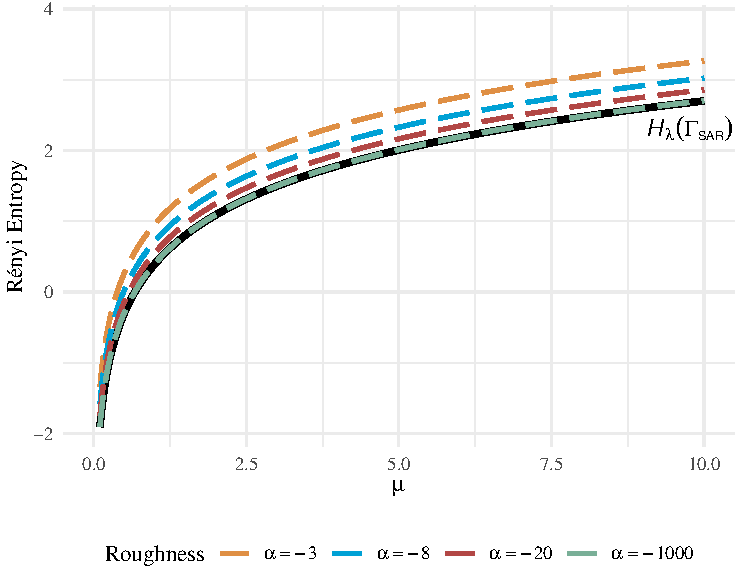
\includegraphics[width=0.45\textwidth,height=\textheight]{R0-Renyi-Entropy-Based-Heterogeneity_files/figure-pdf/fig-plot-1.pdf}

}

\caption{\label{fig-plot}\(H_{\lambda}(\mathcal{G}^0_I)\) converges to
the \(H_{\lambda}(\Gamma_{\text{SAR}})\) when \(\alpha\to-\infty\), with
\(L=8\) and \(\lambda=0.8\).}

\end{figure}%

\subsection{Nonparametric Estimation of Rényi
Entropy}\label{nonparametric-estimation-of-ruxe9nyi-entropy}

Nonparametric estimation of \(H(Z)\) has been widely studied using
spacing-based estimators, which rely on differences between order
statistics
\citeproc{ref-vasicek1976test}{{[}16{]}}--\citeproc{ref-AlOmari2019}{{[}19{]}}.
Recently, Al-Labadi et al.~\citeproc{ref-AlLabadi2024}{{[}20{]}}
proposed a nonparametric estimator for Rényi entropy following this
approach.

Let \(\bm{Z}=(Z_1, Z_2,\ldots,Z_n)\) be an independent and identically
distributed random sample of size \(n\) from a distribution \(F\), and
let \(Z_{(1)} \leq Z_{(2)} \leq \dots \leq Z_{(n)}\) denote its order
statistics. The \(m\)-spacing density estimator is defined as: \[
f_n(Z_{(i)}) = \frac{c_i m / n}{Z_{(i+m)} - Z_{(i-m)}},
\] where \(Z_{(i-m)} = Z_{(1)}\) when \(i \leq m\), and
\(Z_{(i+m)} = Z_{(n)}\) if \(i \geq n - m\). The coefficient \(c_i\) is
given by: \[
c_i = 
\begin{cases}
\frac{m + i - 1}{m}, & \text{if } 1 \leq i \leq m, \\%[6pt]
2, & \text{if } m+1 \leq i \leq n - m, \\%[6pt]
\frac{n + m - i}{m}, & \text{if } n - m + 1 \leq i \leq n.
\end{cases}
\]

Following Vasicek \citeproc{ref-vasicek1976test}{{[}16{]}} and Ebrahimi
et al. \citeproc{ref-Ebrahimi1994}{{[}17{]}} for Shannon entropy
estimation, and using the \(m\)-spacing density estimator, the Rényi
entropy can be estimated as: \begin{align}
\label{eq:est_R}
\widehat{H}_\lambda(\bm{Z}) = \frac{1}{1 - \lambda} \ln \left[\frac{1}{n} \sum_{i=1}^{n} \left( \frac{c_i m / n}{Z_{(i+m)} - Z_{(i-m)}} \right)^{\lambda - 1} \right].
\end{align} This estimator is asymptotically consistent, i.e., it
converges in probability to the true value when \(m,n\rightarrow\infty\)
and \(m/n\rightarrow0\). We choose to use the heuristic formula for
spacing, \(m=\left[\sqrt{n}+0.5\right]\).

\section{PROPOSED METHODOLOGY}\label{sec:met}

\subsection{\texorpdfstring{On \(\lambda\) optimality for a sample
size}{On \textbackslash lambda optimality for a sample size}}\label{on-lambda-optimality-for-a-sample-size}

We aim to determine the optimal order \(\lambda\) for the Rényi entropy
estimator for a sample size \(n=49\). To identify this optimal value, we
analyze both the mean squared error (MSE) and bias of the estimator
across different values of \(\lambda\). Lower MSE and bias indicate
better performance of the estimator in approximating the true entropy.

Based on the results, we find that the optimal value is
\(\lambda = 0.9\), as it minimizes the MSE while maintaining a low bias.
This choice is the same for \(L > 1\). However, for \(L = 1\), the
optimal \(\lambda\) tends to be higher (e.g., \(\lambda = 3\)) to
achieve good results. Fig.~\ref{fig-plotf} illustrates the case for
\(L = 5\).

\begin{figure}[hbt]

\centering{

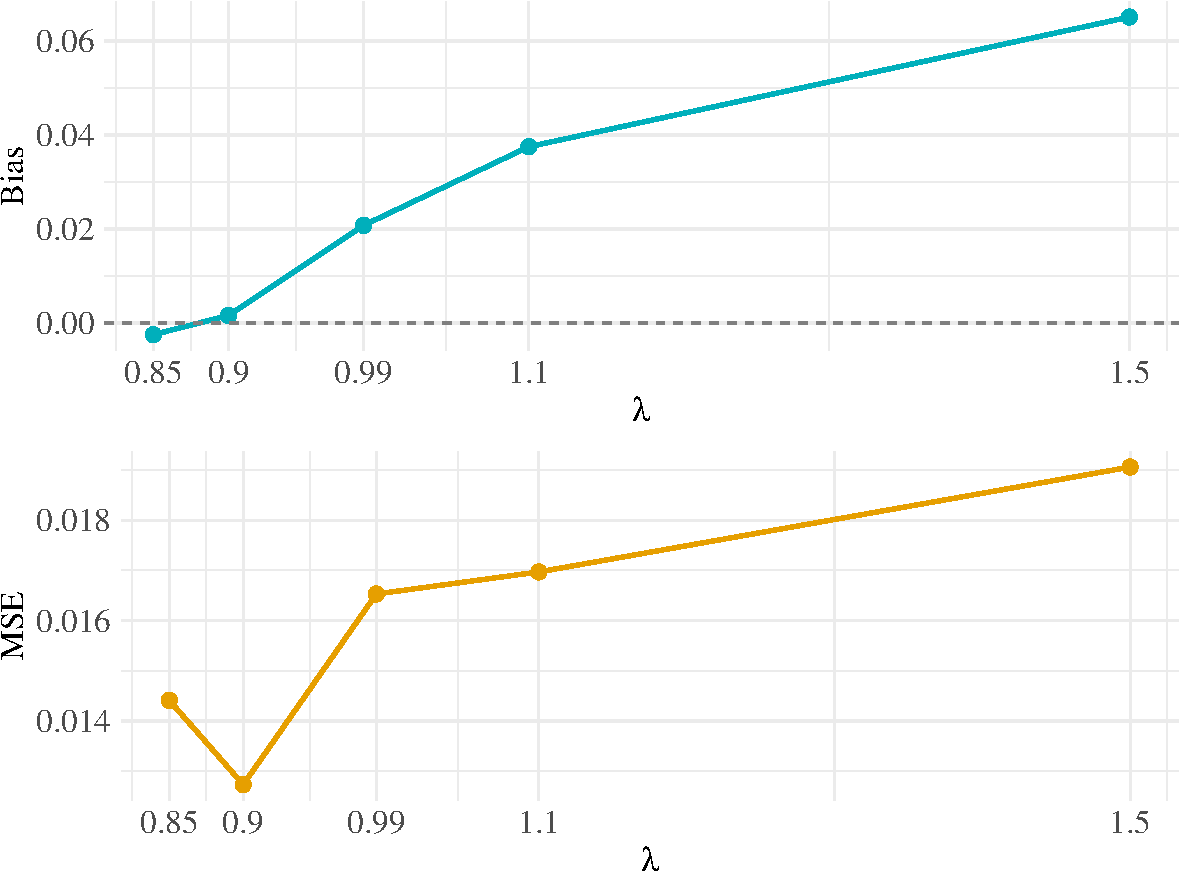
\includegraphics[width=0.42\textwidth,height=\textheight]{R0-Renyi-Entropy-Based-Heterogeneity_files/figure-pdf/fig-plotf-1.pdf}

}

\caption{\label{fig-plotf}Bias and MSE as a function of \(\lambda\),
with \(n=49\), \(L=5\).}

\end{figure}%

\subsection{Bootstrap Correction for Entropy
Estimator}\label{bootstrap-correction-for-entropy-estimator}

Following Refs.~\citeproc{ref-Frery2024}{{[}12{]}},
\citeproc{ref-Alpala2024}{{[}21{]}}, we also refine the non-parametric
entropy estimator \(\widehat{H}_{\lambda}\) in \eqref{eq:est_R} using
the bootstrap technique to reduce its bias and apply the improved
version, denoted as \(\widetilde{H}_{\lambda}\): \[
\widetilde{H}_{\lambda} = 2\widehat{H}_{\lambda}(\bm{Z}) - \frac{1}{B} \sum_{b=1}^{B} \widehat{H}_{\lambda}(\bm{Z}^{(b)}),
\] where \(B\) is the number of bootstrap replications, and
\(\bm{Z}^{(b)}\) is the \(b\)-th resampled dataset obtained by drawing
\(n\) observations with replacement from \(\bm{Z}\).

A Monte Carlo study with \(1,000\) samples from \(\Gamma_{\text{SAR}}\)
(\(\mu = 1\), \(L=5\), \(\lambda = 0.9\)), using \(B = 200\)
replications, confirms that the bootstrap-corrected estimator
\(\widetilde{H}_{\lambda}\) outperforms the original
\(\widehat{H}_{\lambda}\) by reducing both bias and MSE for small sample
sizes, as shown in Fig.~\ref{fig-Plot_bias_msef3}.

\begin{figure}[hbt]

\centering{

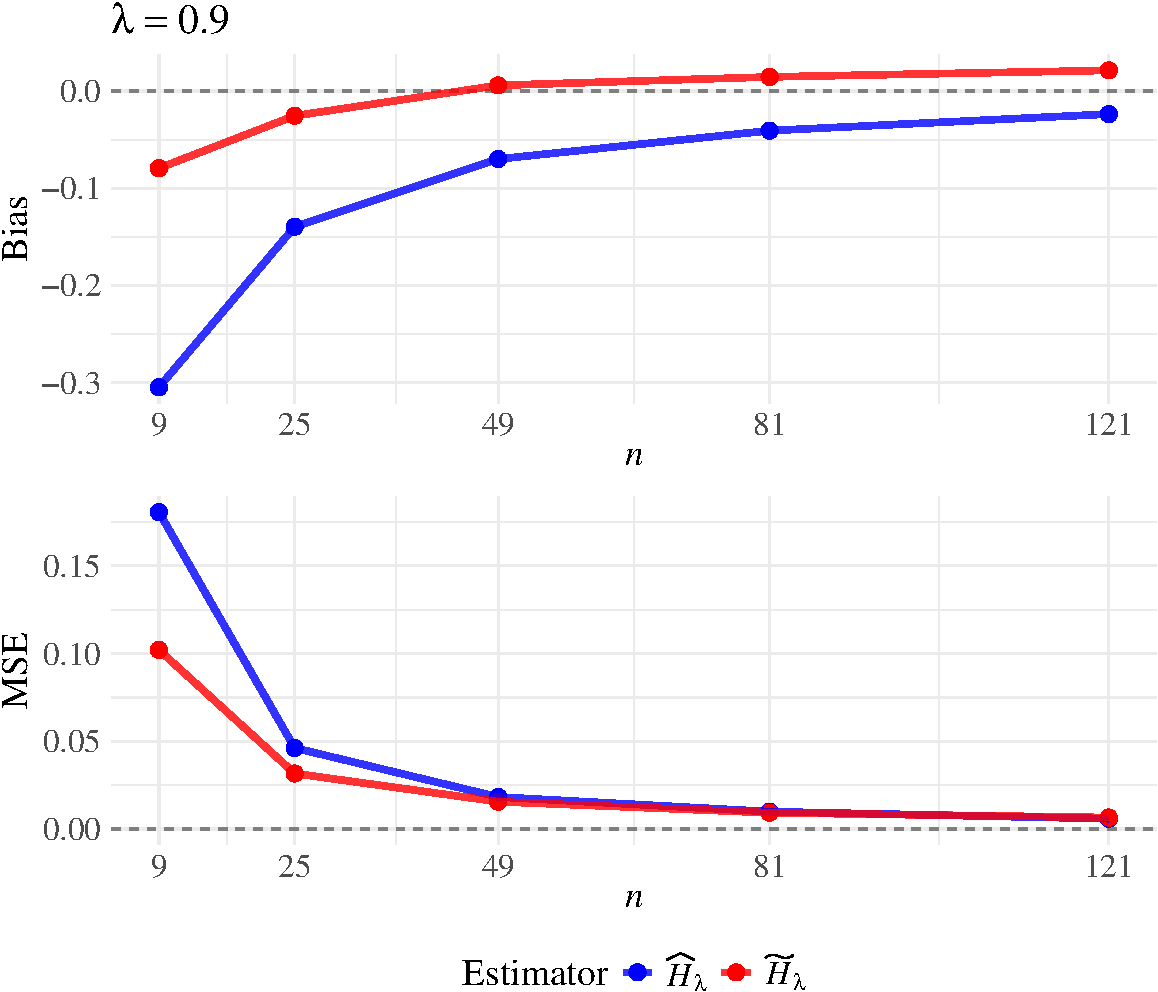
\includegraphics[width=0.42\textwidth,height=\textheight]{R0-Renyi-Entropy-Based-Heterogeneity_files/figure-pdf/fig-Plot_bias_msef3-1.pdf}

}

\caption{\label{fig-Plot_bias_msef3}Bias and MSE of the Rényi entropy
estimators for \(\Gamma_{\text{SAR}}\).}

\end{figure}%

For subsequent simulations we use the \(\widetilde{H}_{\lambda}\)
estimator.

\subsection{Hypothesis Testing}\label{hypothesis-testing}

We test whether the observed data come from a homogeneous
(\(\Gamma_{\text{SAR}}\)) or a heterogeneous (\(\mathcal{G}^0_I\))
region, as follows: \begin{equation}\label{eq:hypothesis_test}
\begin{cases}
\mathcal{H}_0: \mathbb{E}[\widetilde{H}_{\lambda}] = H_{\lambda}(\Gamma_{\text{SAR}}), & \text{(Homogeneous region)} \\[6pt]
\mathcal{H}_1: \mathbb{E}[\widetilde{H}_{\lambda}] = H_{\lambda}(\mathcal{G}^0_I), & \text{(Heterogeneous region)}
\end{cases}
\end{equation}

Under \(\mathcal{H}_0\), the expected value of the entropy estimator
should match the theoretical \(H_{\lambda}(\Gamma_{\text{SAR}})\). If
the estimated entropy significantly deviates from its expected value, we
reject \(\mathcal{H}_0\), indicating the presence of heterogeneity.

Since homogeneity corresponds to \(\alpha \to -\infty\) in the
\(\mathcal{G}^0_I\) model, classical inference methods are inapplicable.
Instead, we propose a test statistic based on the Rényi entropy
estimator, comparing it with its theoretical expectation under
\(\mathcal{H}_0\) to distinguish between homogeneous and heterogeneous
areas.

\subsection{The Proposed Test}\label{the-proposed-test}

Assume we have an estimator \(\widetilde{H}_{\lambda}\) for the Rényi
entropy of an arbitrary model. For testing \eqref{eq:hypothesis_test},
this estimator is expected to be close to the theoretical expression
given in Equation \eqref{eq-HGammaSAR}. Since \(L\geq1\) is known, we
define the test statistic as follows: \begin{multline}
\label{eq-test}
S(\bm{Z}; L) = \widetilde{H}_{\lambda} - \bigl\{\ln \widehat{\mu} - \ln L + \frac{1}{1-\lambda}
\bigl[-\lambda\,\ln\Gamma(L) \\  
+ \ln\Gamma\bigl(\lambda(L-1)+1\bigr)  
- \bigl(\lambda(L-1)+1\bigr)\,\ln\lambda
\bigr]\bigr\}.
\end{multline} where
\(\ln \widehat{\mu}={\textstyle\frac{1}{n}\sum_{i=1}^n Z_{i}}\) is the
natural logarithm of the sample mean.

When the null hypothesis holds, this test statistic is expected to be
close to zero. For illustrative purposes,
Fig.~\ref{fig-density_entropyR} shows the empirical density of
\(S(\bm{Z}; L)\), based on \(10,000\) simulations of the
\(\Gamma_{\text{SAR}}\) model, with \(\lambda=0.9\) and
\(L \in \{5,18\}\).

\begin{figure}[hbt]

\centering{

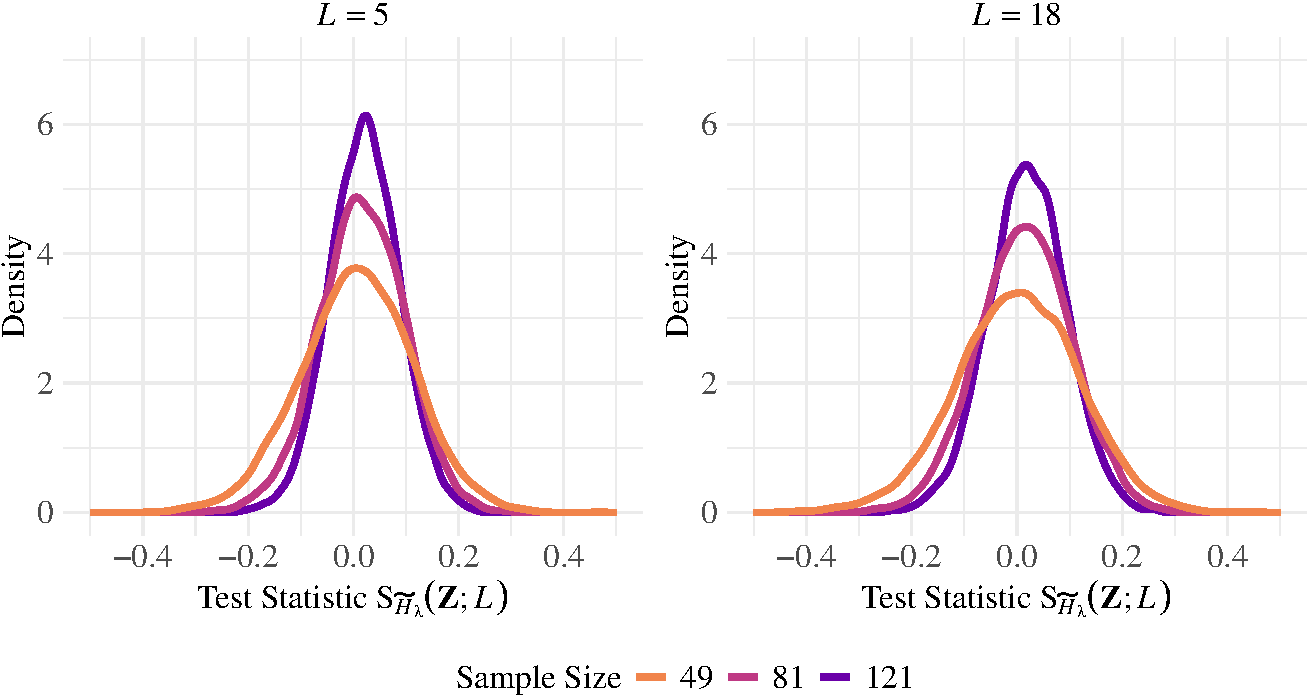
\includegraphics[width=0.47\textwidth,height=\textheight]{R0-Renyi-Entropy-Based-Heterogeneity_files/figure-pdf/fig-density_entropyR-1.pdf}

}

\caption{\label{fig-density_entropyR}Empirical densities of
\(S_{\widetilde{H}_{\lambda}}(\bm{Z}; L)\) under \(\mathcal{H}_0\).}

\end{figure}%

Under the asymptotic properties of the entropy
estimator~\citeproc{ref-vasicek1976test}{{[}16{]}}, for sufficiently
large samples, \(S(\bm{Z}; L)\) follows an asymptotic normal
distribution: \begin{equation*}
S(\bm{Z}; L) \overset{d}{\longrightarrow} \mathcal{N}(\mu_S,\,\sigma^{2})\,.
\end{equation*} We define the standardized test statistic:
\begin{equation*}
\varepsilon = \frac{S(\bm{Z}; L) - \hat{\mu}_S}{\hat{\sigma}_S},
\end{equation*} where \(\hat{\mu}_S = \mathbb{E}[S(\bm{Z}; L)]\) and
\(\hat{\sigma}_S = \sqrt{\text{Var}[S(\bm{Z}; L)]}\). By the central
limit theorem, under the null hypothesis, \(\varepsilon\) asymptotically
follows a standard normal distribution: \begin{equation*}
\varepsilon \overset{d}{\longrightarrow} \mathcal{N}(0,1)\,,
\end{equation*} where \(d\) represents convergence in distribution.
Fig.~\ref{fig-density_entropyR} presents the behavior of the empirical
distribution of the standardized test statistic. Thus, the \(p\)-values
are calculated as \(2\Phi(-|\varepsilon|)\), where \(\Phi(\cdot)\) is
the cumulative distribution function of the standard normal
distribution.

\begin{figure}[hbt]

\centering{

\includegraphics[width=0.35\textwidth,height=\textheight]{R0-Renyi-Entropy-Based-Heterogeneity_files/figure-pdf/fig-density_entropyR_standardized0-1.pdf}

}

\caption{\label{fig-density_entropyR_standardized0}Standardized
empirical densities of \(S_{\widetilde{H}_{\lambda}}(\bm{Z}; L)\) under
\(\mathcal{H}_0\).}

\end{figure}%

In general, hypothesis tests aim to achieve a controlled type I error
rate (size) and high test power (sensitivity to departures from
\(\mathcal{H}_0\)). To assess these properties, we performed a Monte
Carlo simulation with \(1000\) replications at significance levels
\(1\%\), \(5\%\), and \(10\%\), evaluating the test under the null
hypothesis (\(\Gamma_{\text{SAR}}\) distribution), varying sample size
and values of \(L\) for \(\mu=1\). The observed type I error rates
aligned with the nominal values, confirming the test validity.

Further, we examined the power under the alternative hypothesis
(\(\mathcal{G}^0_I\) distribution) with \(\mu=1\), \(\lambda=0.9\) and
\(\alpha=-2\). As expected, power improves as the sample size and number
of looks increase, demonstrating the test effectiveness. The results are
shown in Table \ref{tab:table_size_power}.

\begin{table}[htb]
\centering\centering
\caption{\label{tab:table_size_power}Size and Power of the $S_{\widetilde{H}_{\lambda}}(\bm{Z})$ test statistic.}
\resizebox{\ifdim\width>\linewidth\linewidth\else\width\fi}{!}{
\fontsize{7}{9}\selectfont
\begin{tabu} to \linewidth {>{\centering}X>{\centering}X>{\centering}X>{\centering}X>{\centering}X>{\centering}X>{\centering}X>{\centering}X}
\toprule
\multicolumn{1}{c}{ } & \multicolumn{1}{c}{ } & \multicolumn{3}{c}{Size} & \multicolumn{3}{c}{Power} \\
\cmidrule(l{3pt}r{3pt}){3-5} \cmidrule(l{3pt}r{3pt}){6-8}
\multicolumn{1}{c}{$\bm{L}$} & \multicolumn{1}{c}{$\bm{n}$} & \multicolumn{1}{c}{$\bm{1\%}$} & \multicolumn{1}{c}{$\bm{5\%}$} & \multicolumn{1}{c}{$\bm{10\%}$} & \multicolumn{1}{c}{$\bm{1\%}$} & \multicolumn{1}{c}{$\bm{5\%}$} & \multicolumn{1}{c}{$\bm{10\%}$}\\
\midrule
 & 25 & $\phantom{-}0.014$ & $\phantom{-}0.050$ & $\phantom{-}0.100$ & $\phantom{-}0.978$ & $\phantom{-}0.994$ & $\phantom{-}0.993$\\

 & 49 & $\phantom{-}0.011$ & $\phantom{-}0.048$ & $\phantom{-}0.109$ & $\phantom{-}0.994$ & $\phantom{-}1.000$ & $\phantom{-}0.999$\\

 & 81 & $\phantom{-}0.012$ & $\phantom{-}0.057$ & $\phantom{-}0.103$ & $\phantom{-}0.998$ & $\phantom{-}0.998$ & $\phantom{-}0.999$\\

\multirow{-4}{*}[\normalbaselineskip]{\centering\arraybackslash 5} & 121 & $\phantom{-}0.013$ & $\phantom{-}0.061$ & $\phantom{-}0.116$ & $\phantom{-}0.999$ & $\phantom{-}0.999$ & $\phantom{-}0.997$\\
\cmidrule{1-8}
 & 25 & $\phantom{-}0.010$ & $\phantom{-}0.051$ & $\phantom{-}0.105$ & $\phantom{-}0.996$ & $\phantom{-}0.999$ & $\phantom{-}1.000$\\

 & 49 & $\phantom{-}0.008$ & $\phantom{-}0.056$ & $\phantom{-}0.109$ & $\phantom{-}1.000$ & $\phantom{-}0.999$ & $\phantom{-}1.000$\\

 & 81 & $\phantom{-}0.012$ & $\phantom{-}0.052$ & $\phantom{-}0.097$ & $\phantom{-}0.999$ & $\phantom{-}0.999$ & $\phantom{-}0.999$\\

\multirow{-4}{*}[\normalbaselineskip]{\centering\arraybackslash 8} & 121 & $\phantom{-}0.016$ & $\phantom{-}0.070$ & $\phantom{-}0.116$ & $\phantom{-}0.998$ & $\phantom{-}1.000$ & $\phantom{-}0.999$\\
\cmidrule{1-8}
 & 25 & $\phantom{-}0.016$ & $\phantom{-}0.051$ & $\phantom{-}0.111$ & $\phantom{-}1.000$ & $\phantom{-}1.000$ & $\phantom{-}1.000$\\

 & 49 & $\phantom{-}0.014$ & $\phantom{-}0.047$ & $\phantom{-}0.098$ & $\phantom{-}1.000$ & $\phantom{-}1.000$ & $\phantom{-}1.000$\\

 & 81 & $\phantom{-}0.013$ & $\phantom{-}0.048$ & $\phantom{-}0.106$ & $\phantom{-}1.000$ & $\phantom{-}1.000$ & $\phantom{-}1.000$\\

\multirow{-4}{*}[\normalbaselineskip]{\centering\arraybackslash 18} & 121 & $\phantom{-}0.012$ & $\phantom{-}0.066$ & $\phantom{-}0.110$ & $\phantom{-}1.000$ & $\phantom{-}1.000$ & $\phantom{-}1.000$\\
\bottomrule
\end{tabu}}
\end{table}

\section{Applications to SAR Data}\label{sec:app}

In this section, we evaluate the proposed test statistic on real SAR
data to assess its effectiveness in detecting heterogeneity. The test
was applied to SAR intensity images from several regions: urban,
agricultural, and water. In particular, we analyzed three images: the
first from London, United Kingdom; the second from the surroundings of
Munich, Germany; and the third from Dublin Port, Ireland, as shown in
Figs.~\ref{fig:london}(a), \ref{fig:munich}(a), and \ref{fig:dublin}(a).
Table~\ref{tab:table_param} provides detailed acquisition parameters for
these images. \renewcommand{\arraystretch}{3}

\begin{table}[hbt]
\centering\centering
\caption{\label{tab:table_param}Parameters of selected SAR images.}
\resizebox{\ifdim\width>\linewidth\linewidth\else\width\fi}{!}{
\fontsize{21}{23}\selectfont
\begin{tabu} to \linewidth {>{\centering\arraybackslash}p{3.0cm}>{\centering\arraybackslash}p{3.7cm}>{\centering\arraybackslash}p{1.5cm}>{\centering\arraybackslash}p{2.5cm}>{\centering\arraybackslash}p{4cm}>{\centering\arraybackslash}p{1.5cm}>{\centering\arraybackslash}p{3.0cm}>{\centering\arraybackslash}p{3.5cm}}
\toprule
\multicolumn{1}{c}{\textbf{Site}} & \multicolumn{1}{c}{\textbf{Mission}} & \multicolumn{1}{c}{\textbf{Band}} & \multicolumn{1}{c}{\textbf{Polarization}} & \multicolumn{1}{c}{\textbf{Size (pixels)}} & \multicolumn{1}{c}{$\bm{L}$} & \multicolumn{1}{c}{\textbf{Resolution [m]} } & \multicolumn{1}{c}{\textbf{Acquisition Date}}\\
\midrule
London & TanDEM-X & X & HH & $2000\times2000$ & $1$ & $0.99/0.99$ & 12-11-2021\\
Munich & UAVSAR & L & HH & $1024\times1024$ & $12$ & $4.9/7.2$ & 16-04-2015\\
Dublin & TanDEM-X & X & HH & $1100\times1100$ & $16$ & $1.35/1.35$ & 03-09-2017\\
\bottomrule
\end{tabu}}
\end{table}

To evaluate the performance of our proposal, we applied the test
statistics \(S_{\widetilde{H}_{\lambda}}(\bm{Z}; L)\) and
\(S_{\widetilde{H}_{\text{AO}}}(\bm{Z}; L)\), based on Shannon entropy
as described in~\citeproc{ref-Frery2024}{{[}12{]}}, using a local
sliding window of size \(7\times7\). The resulting \(p\)-value maps are
presented in Figs.~\ref{fig:london}(b), \ref{fig:london}(d),
\ref{fig:munich}(b), \ref{fig:munich}(d), \ref{fig:dublin}(b), and
\ref{fig:dublin}(d). These maps employ a color gradient, where darker
regions indicate areas with higher roughness, while lighter regions
correspond to smoother, less textured surfaces.

In order to better illustrate the decision-making process of both tests,
binary maps at a significance level of \(0.05\) are shown in
Figs.~\ref{fig:london}(c), \ref{fig:london}(e), \ref{fig:munich}(c),
\ref{fig:munich}(e), \ref{fig:dublin}(c), and \ref{fig:dublin}(e).

In these binary representations, white areas correspond to \(p\)-values
greater than \(0.05\), indicating that there is no statistical evidence
to reject the null hypothesis (homogeneous regions). In contrast, black
areas represent regions where the \(p\)-values are less than \(0.05\),
indicating statistically significant heterogeneity.

The Rényi entropy-based test demonstrated greater sensitivity in
detecting textural variations compared to the Shannon-based approach,
due to the flexibility provided by the parameter \(\lambda\). When
\(\lambda \to 1\), Rényi entropy converges to Shannon entropy, resulting
in similar heterogeneity detection. Our analysis shows that the optimal
\(\lambda\) value depends on the number of looks: for single-look images
like London, \(\lambda = 3\) provided the best contrast, while for
multi-look images like Munich and Dublin, \(\lambda = 0.9\) was more
effective.

\begin{figure*}[hbt]
    \centering
    \begin{subfigure}{0.17\textwidth}
        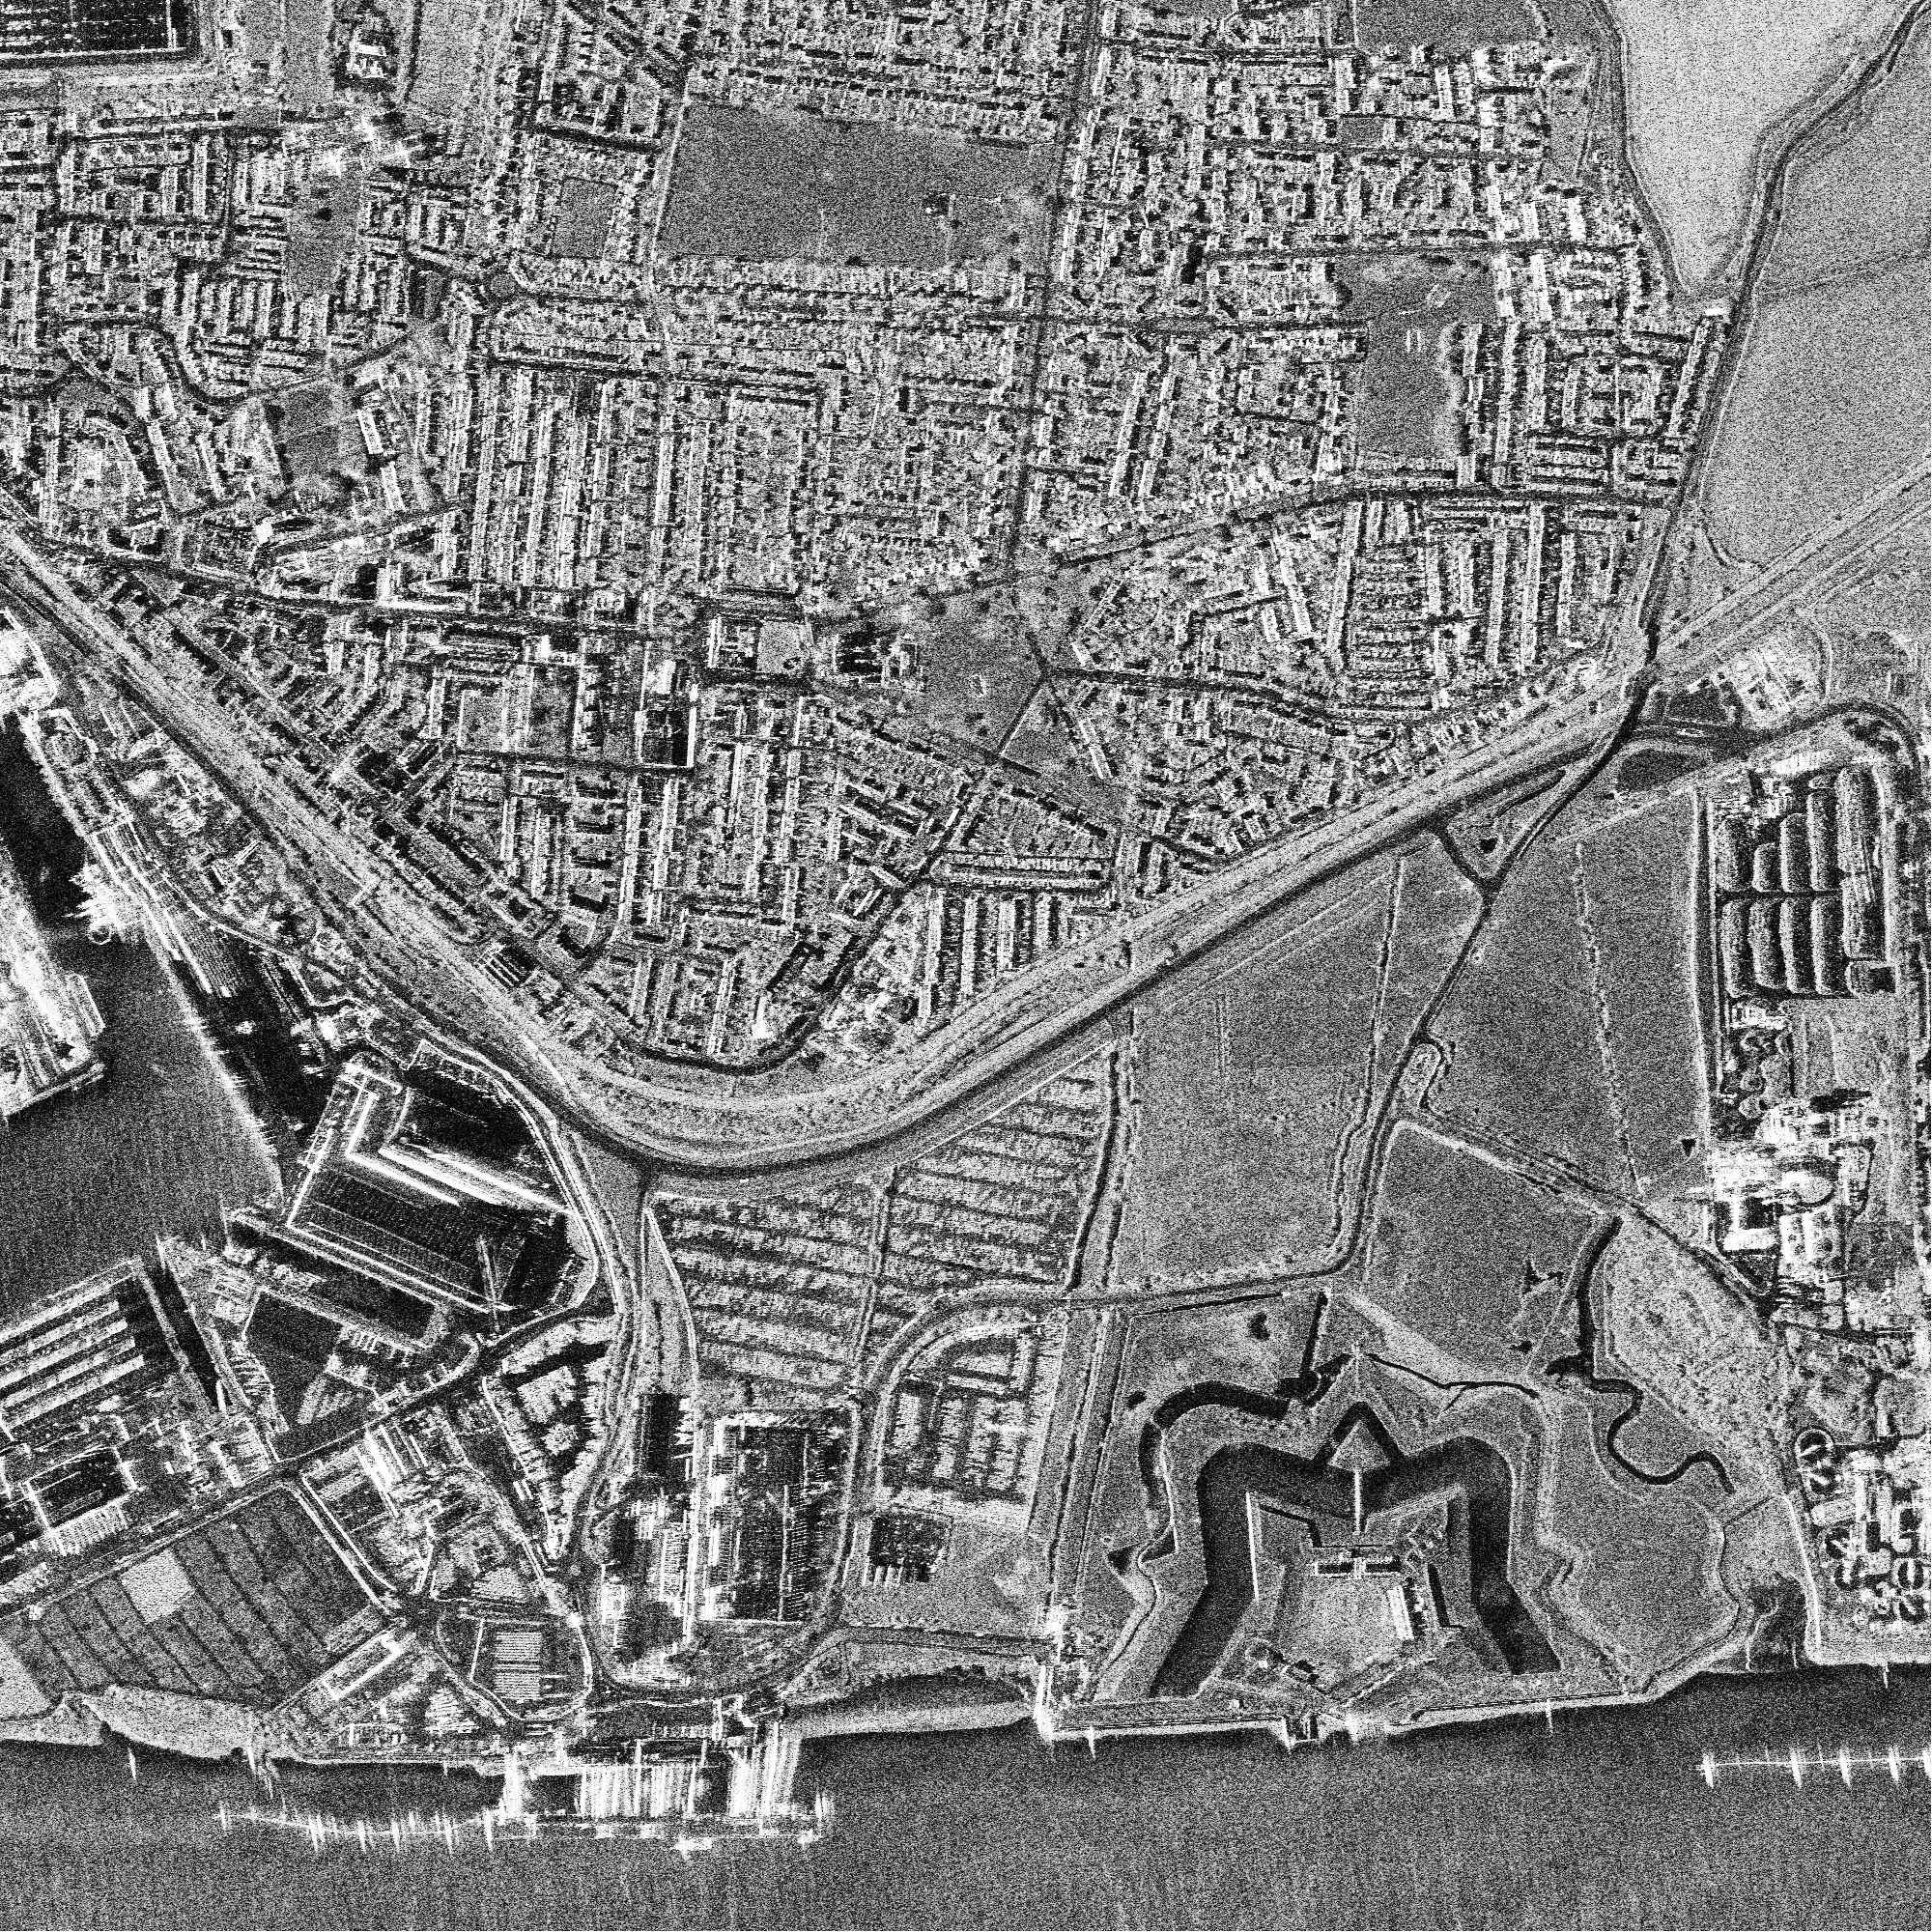
\includegraphics[width=\linewidth]{./Figures/london_2000.png}
        \caption{ SAR image}
        \label{fig:1a}
    \end{subfigure}
    \begin{subfigure}{0.22\textwidth}
        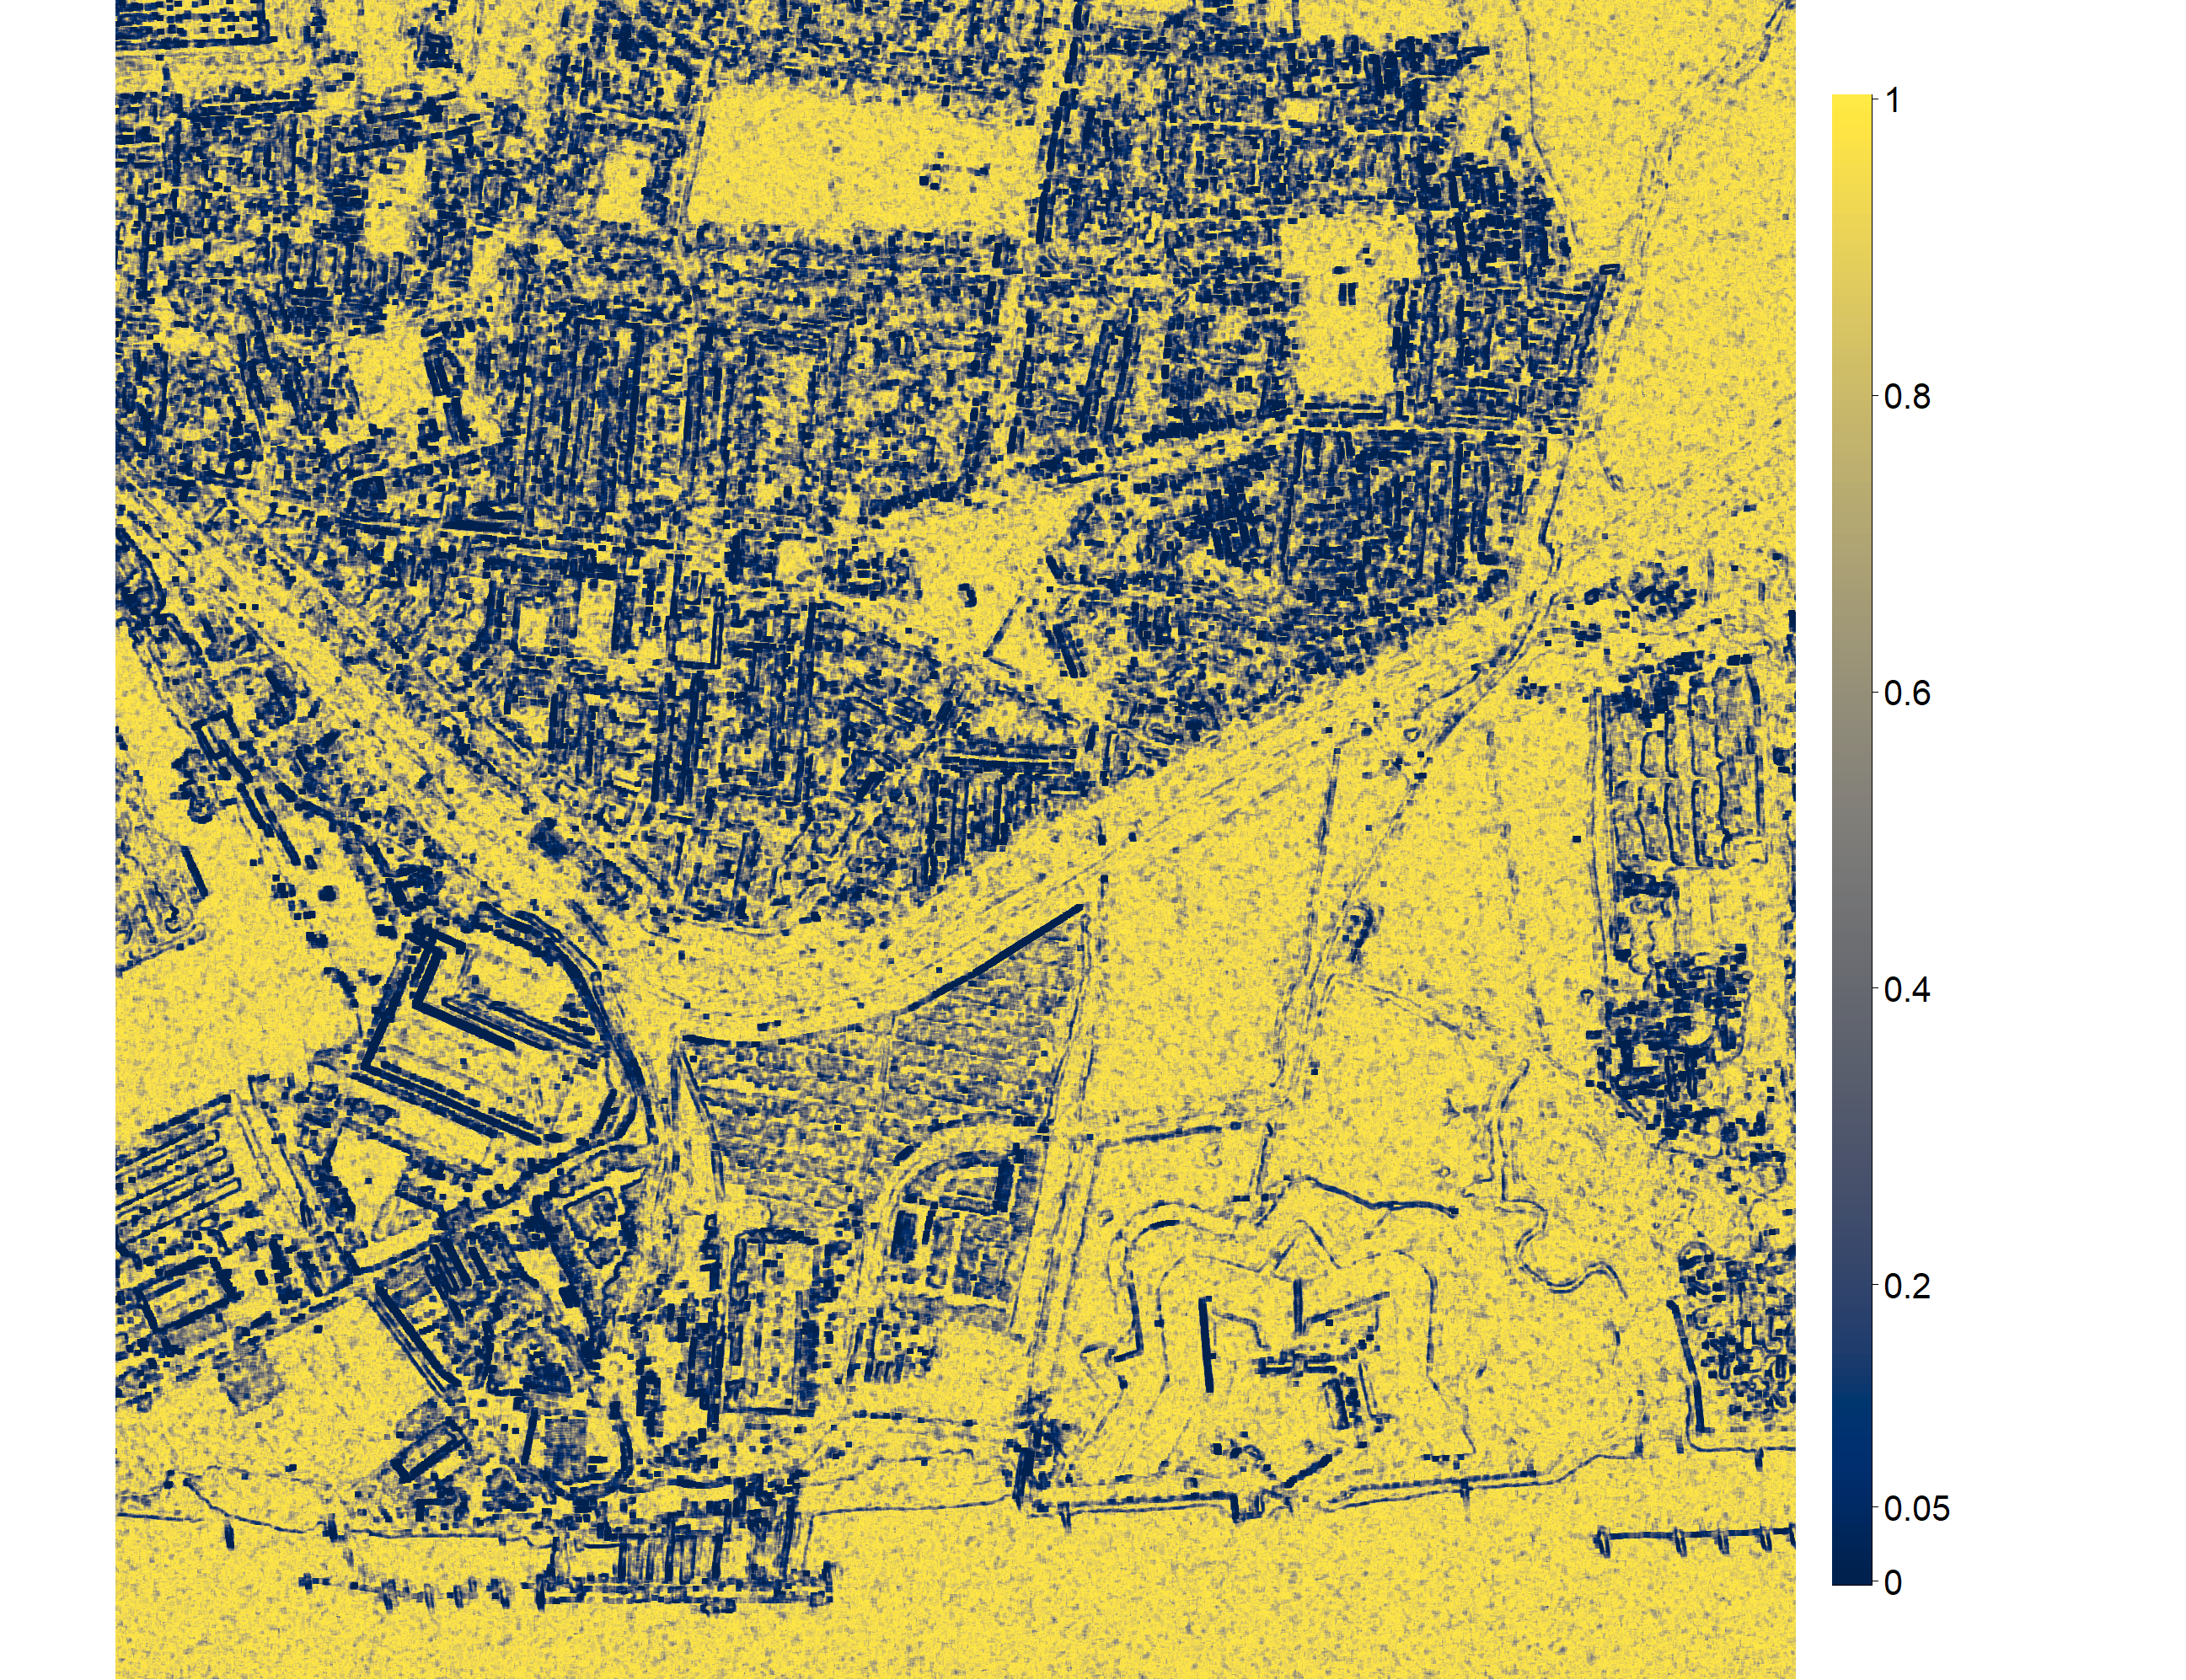
\includegraphics[width=\linewidth]{./Figures/H_pvalue_london_renyi.png}
        \caption{ $p$-values for $\small{S_{\widetilde{H}_{\lambda}}}$}
        \label{fig:1b}
    \end{subfigure}
    \begin{subfigure}{0.17\textwidth}
        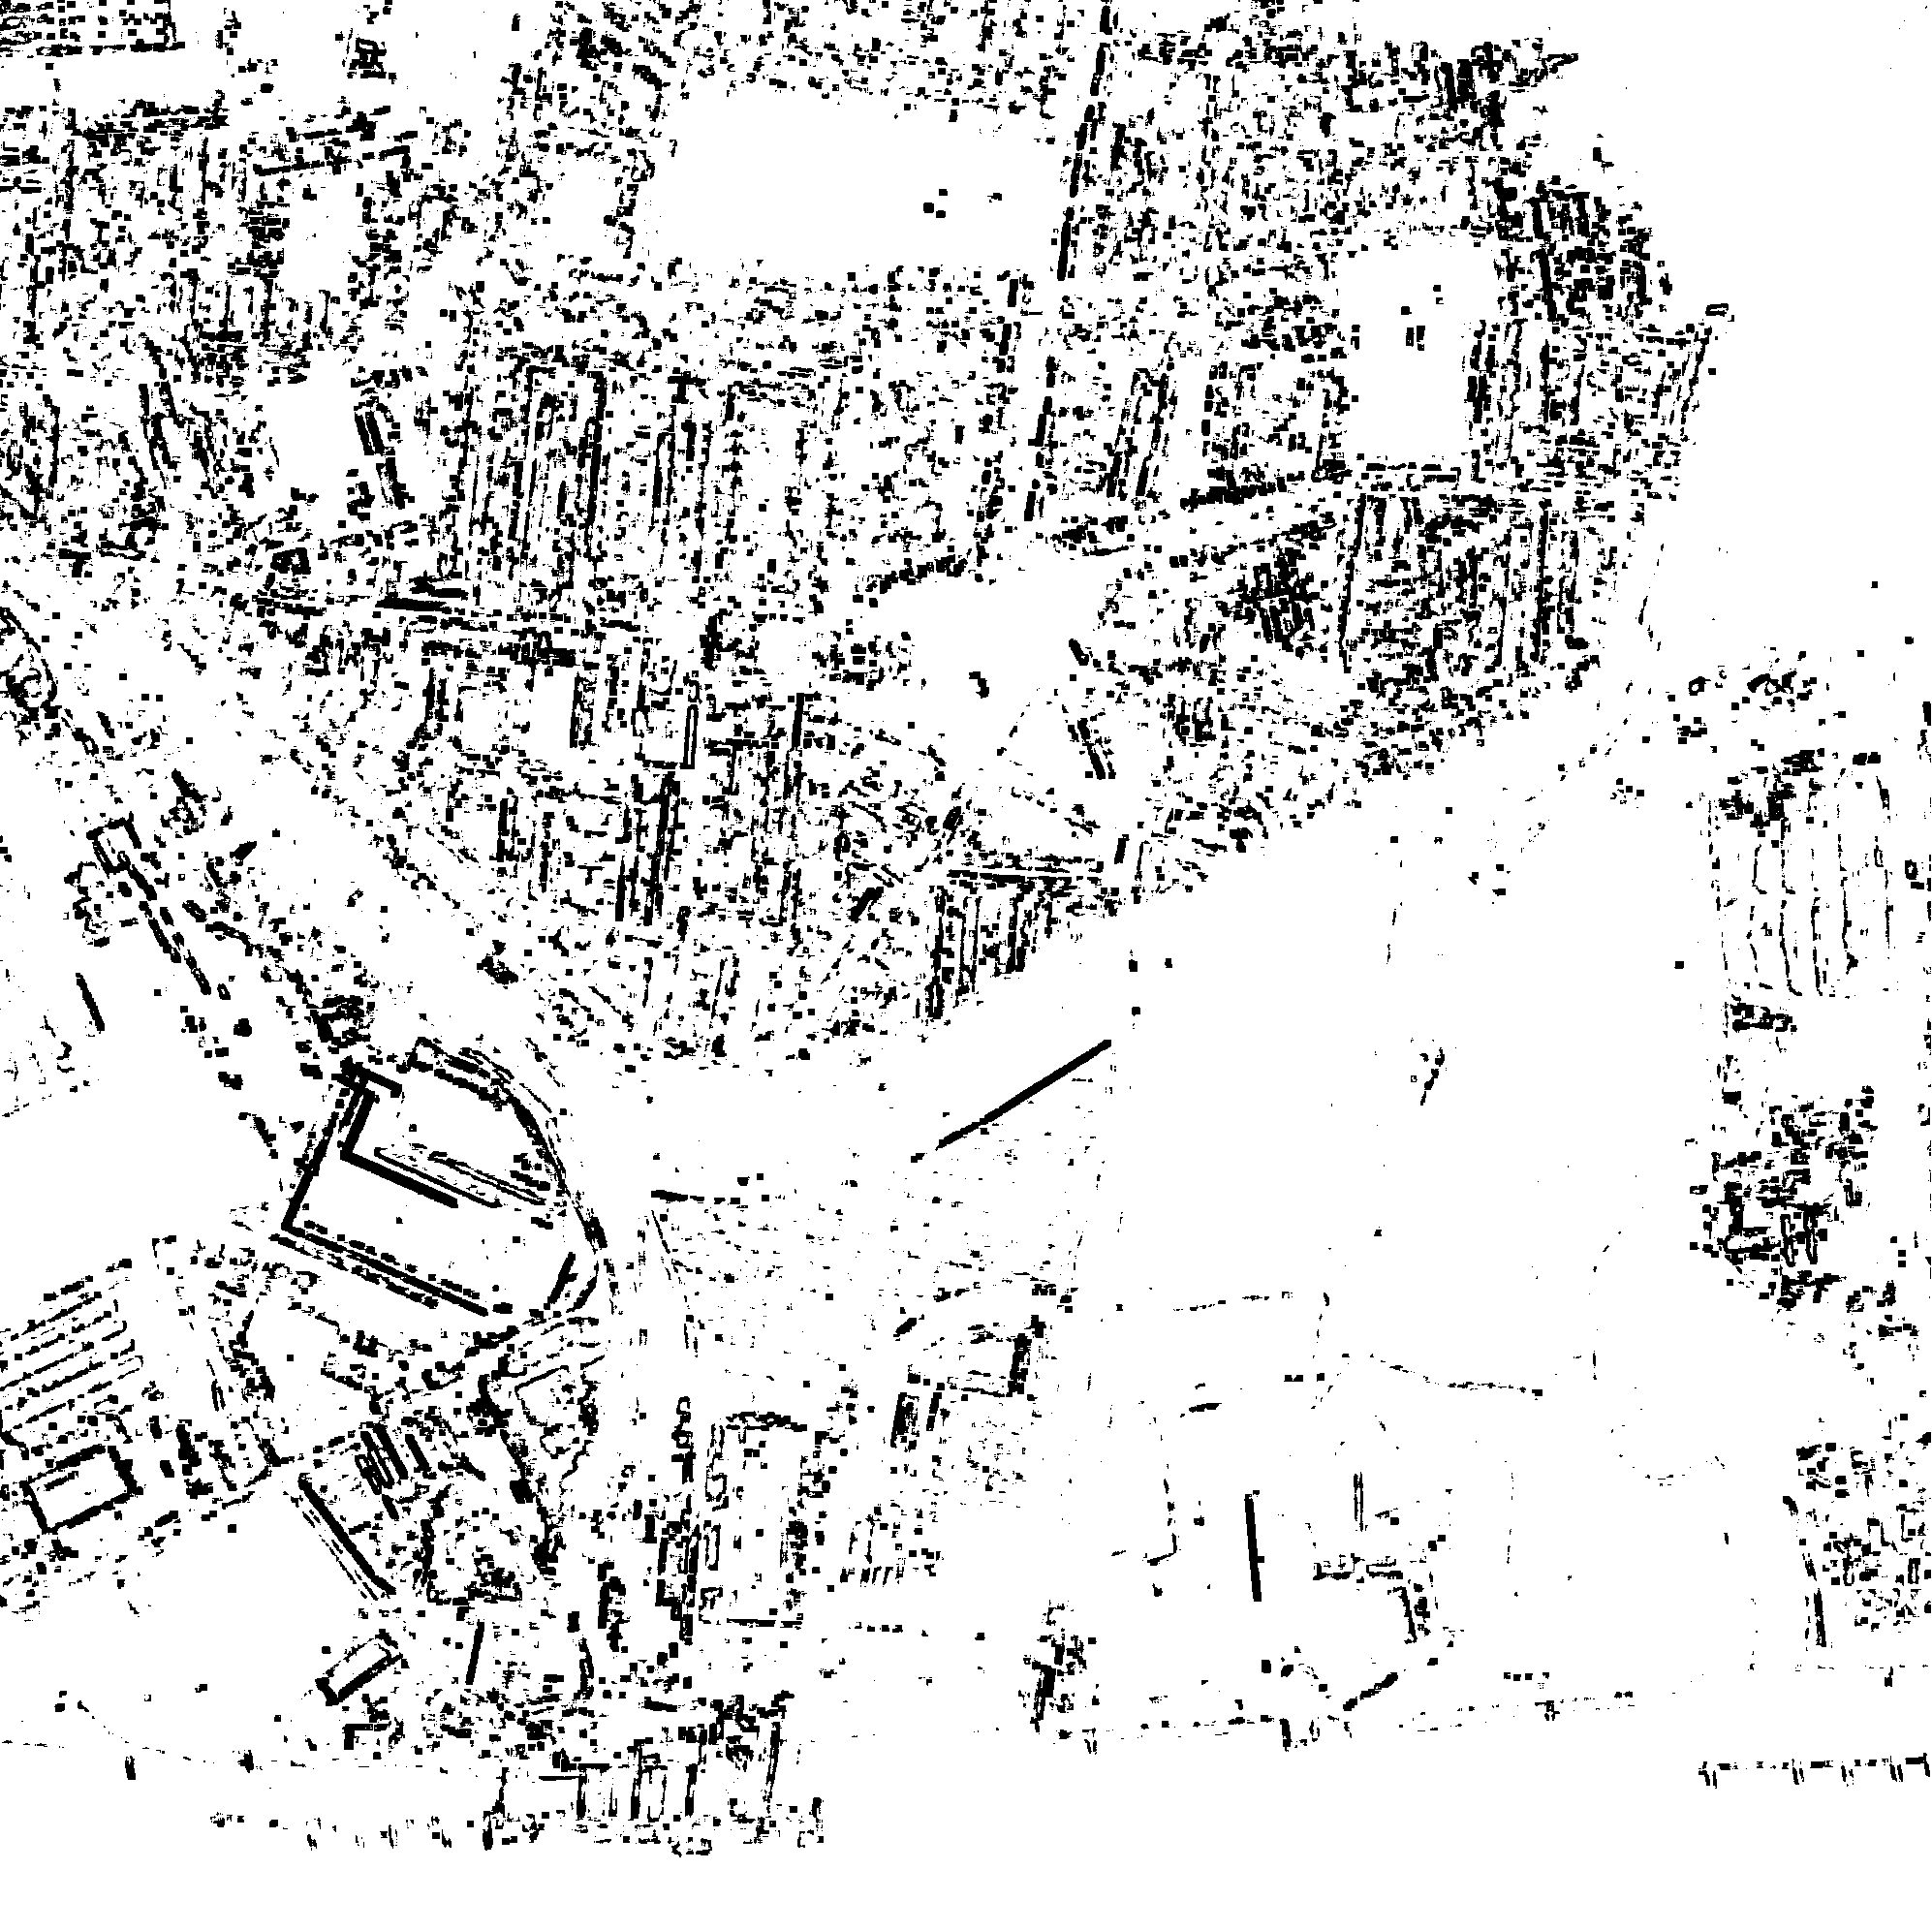
\includegraphics[width=\linewidth]{./Figures/H_005_london_renyi_L1_.png}
        \caption{Binary map for $\small{S_{\widetilde{H}_{\lambda}}}$}
        \label{fig:1c}
    \end{subfigure}
    \begin{subfigure}{0.22\textwidth}
        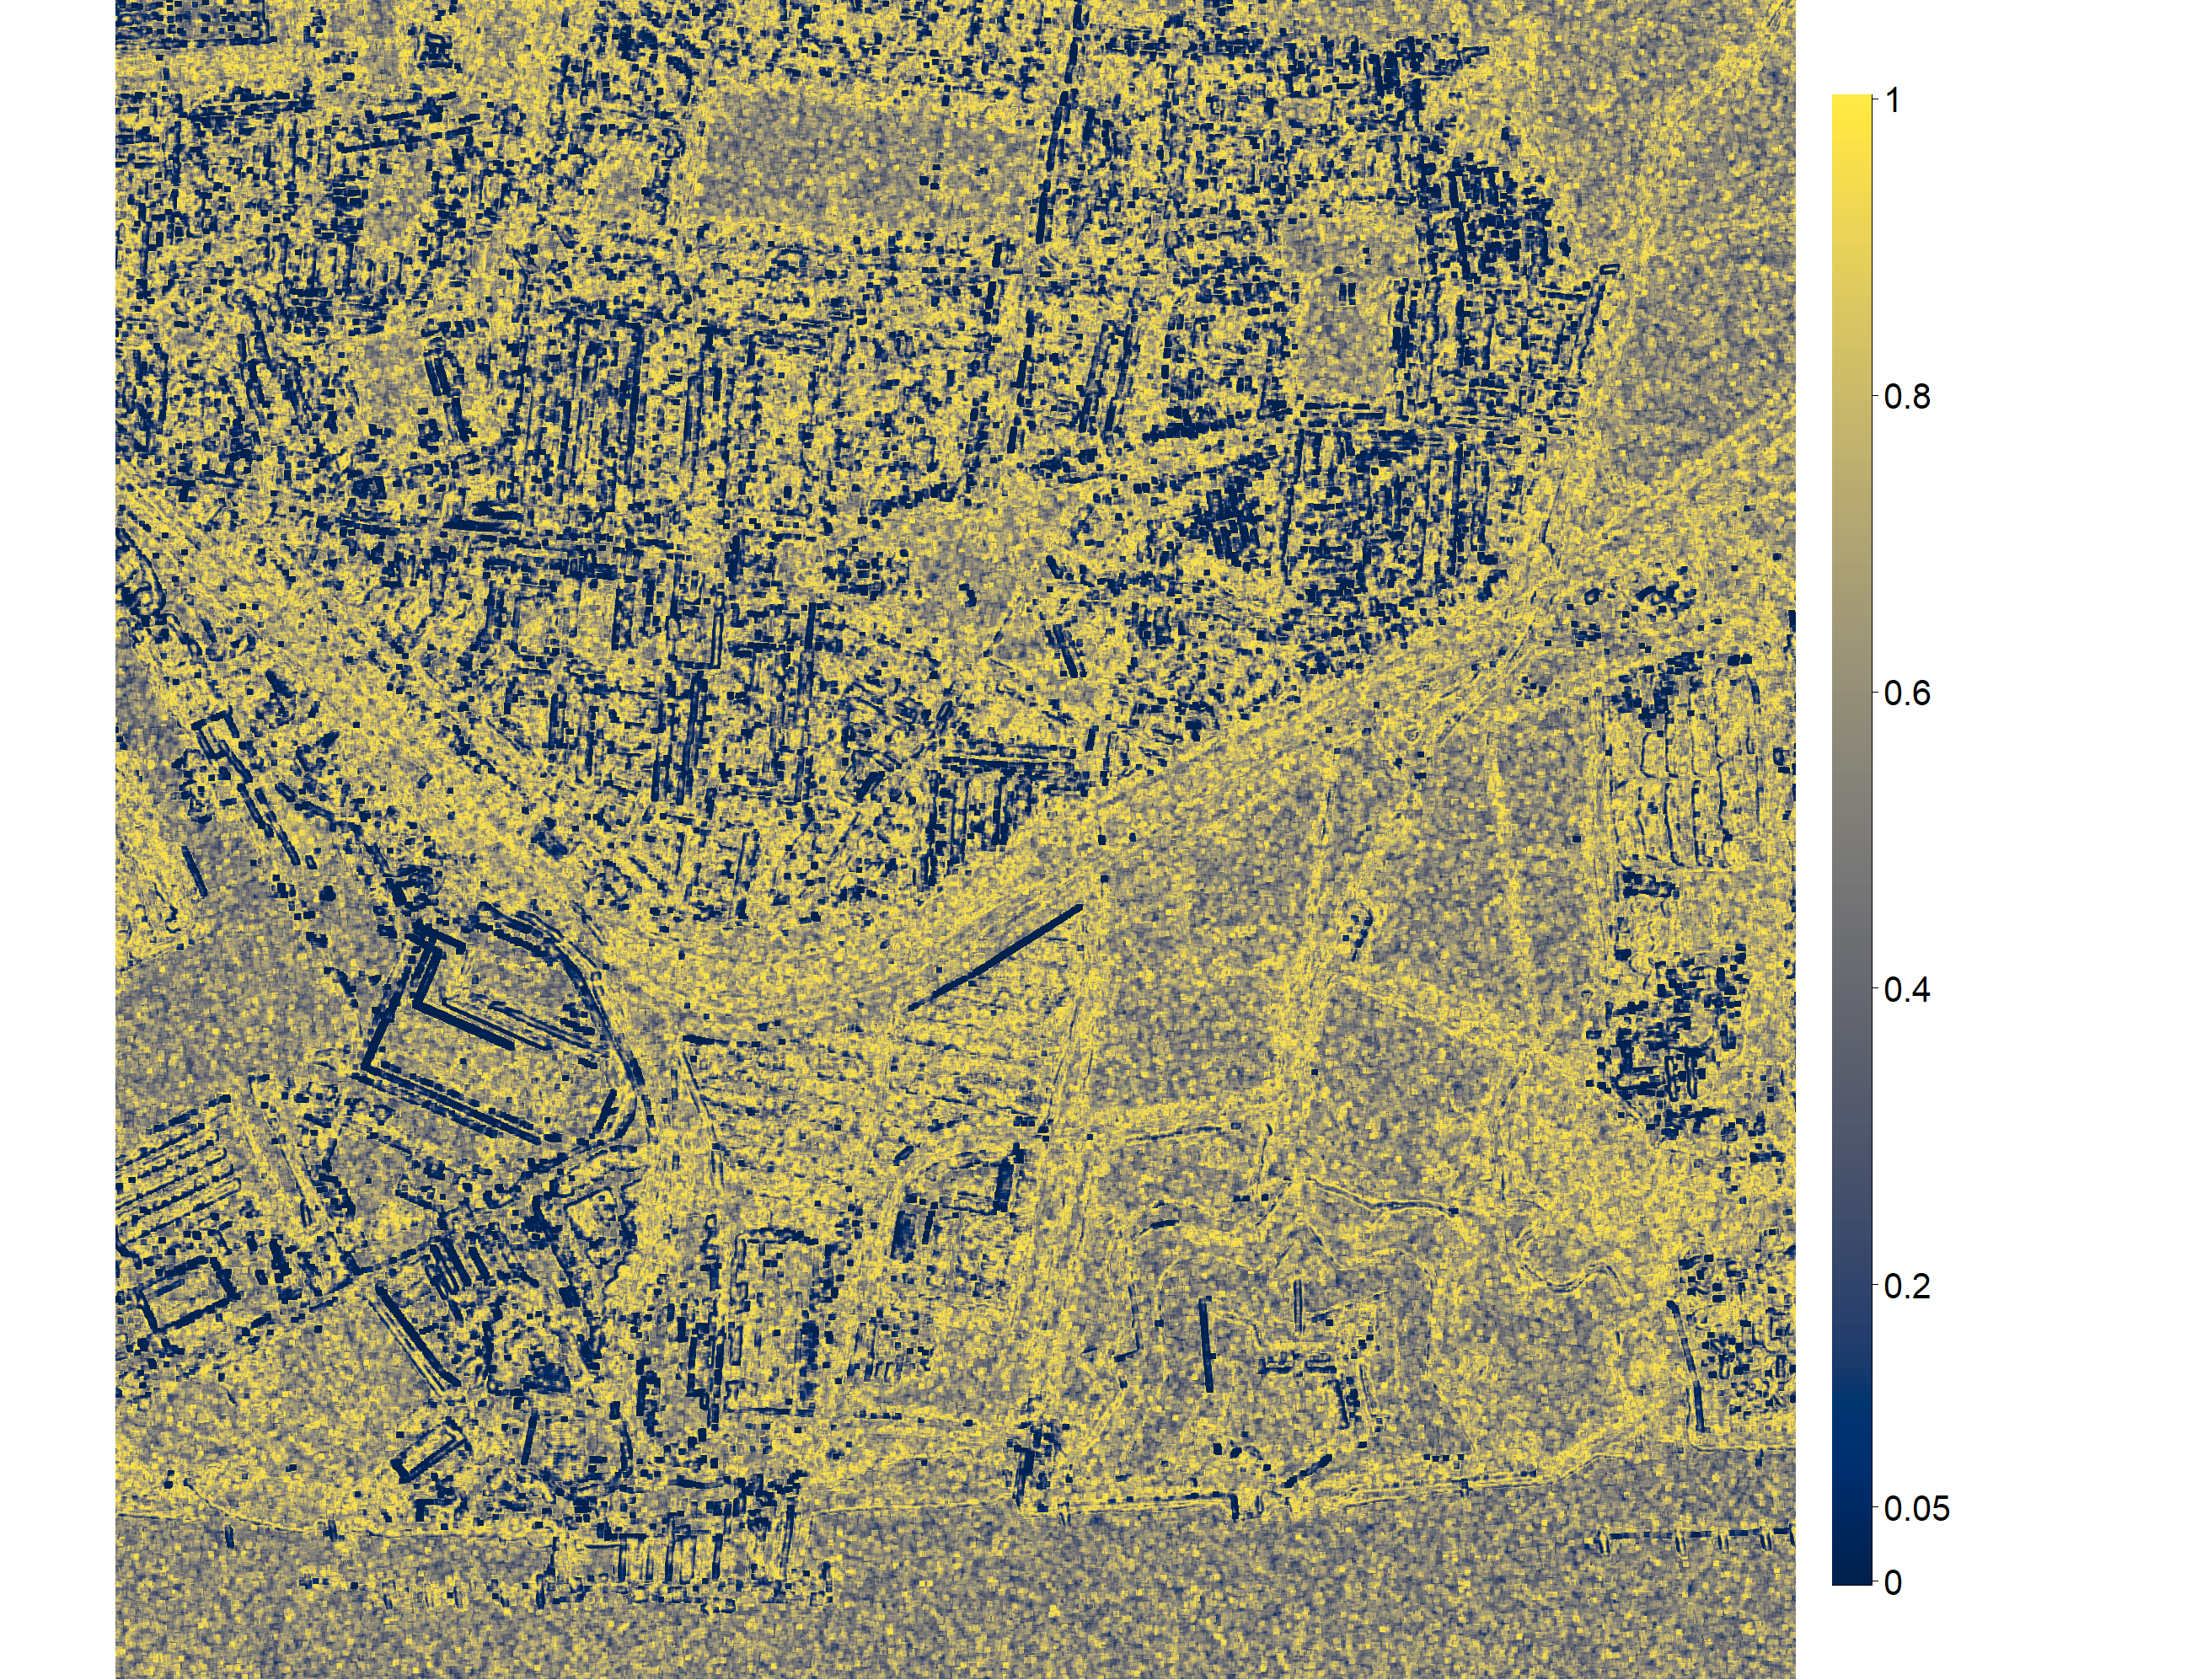
\includegraphics[width=\linewidth]{./Figures/H_pvalue_london_Shannon_c1.png}
        \caption{$p$-values for $\tiny{S_{\widetilde{H}_{\text{AO}}}}$ }
        \label{fig:1d}
    \end{subfigure}
    \begin{subfigure}{0.17\textwidth}
        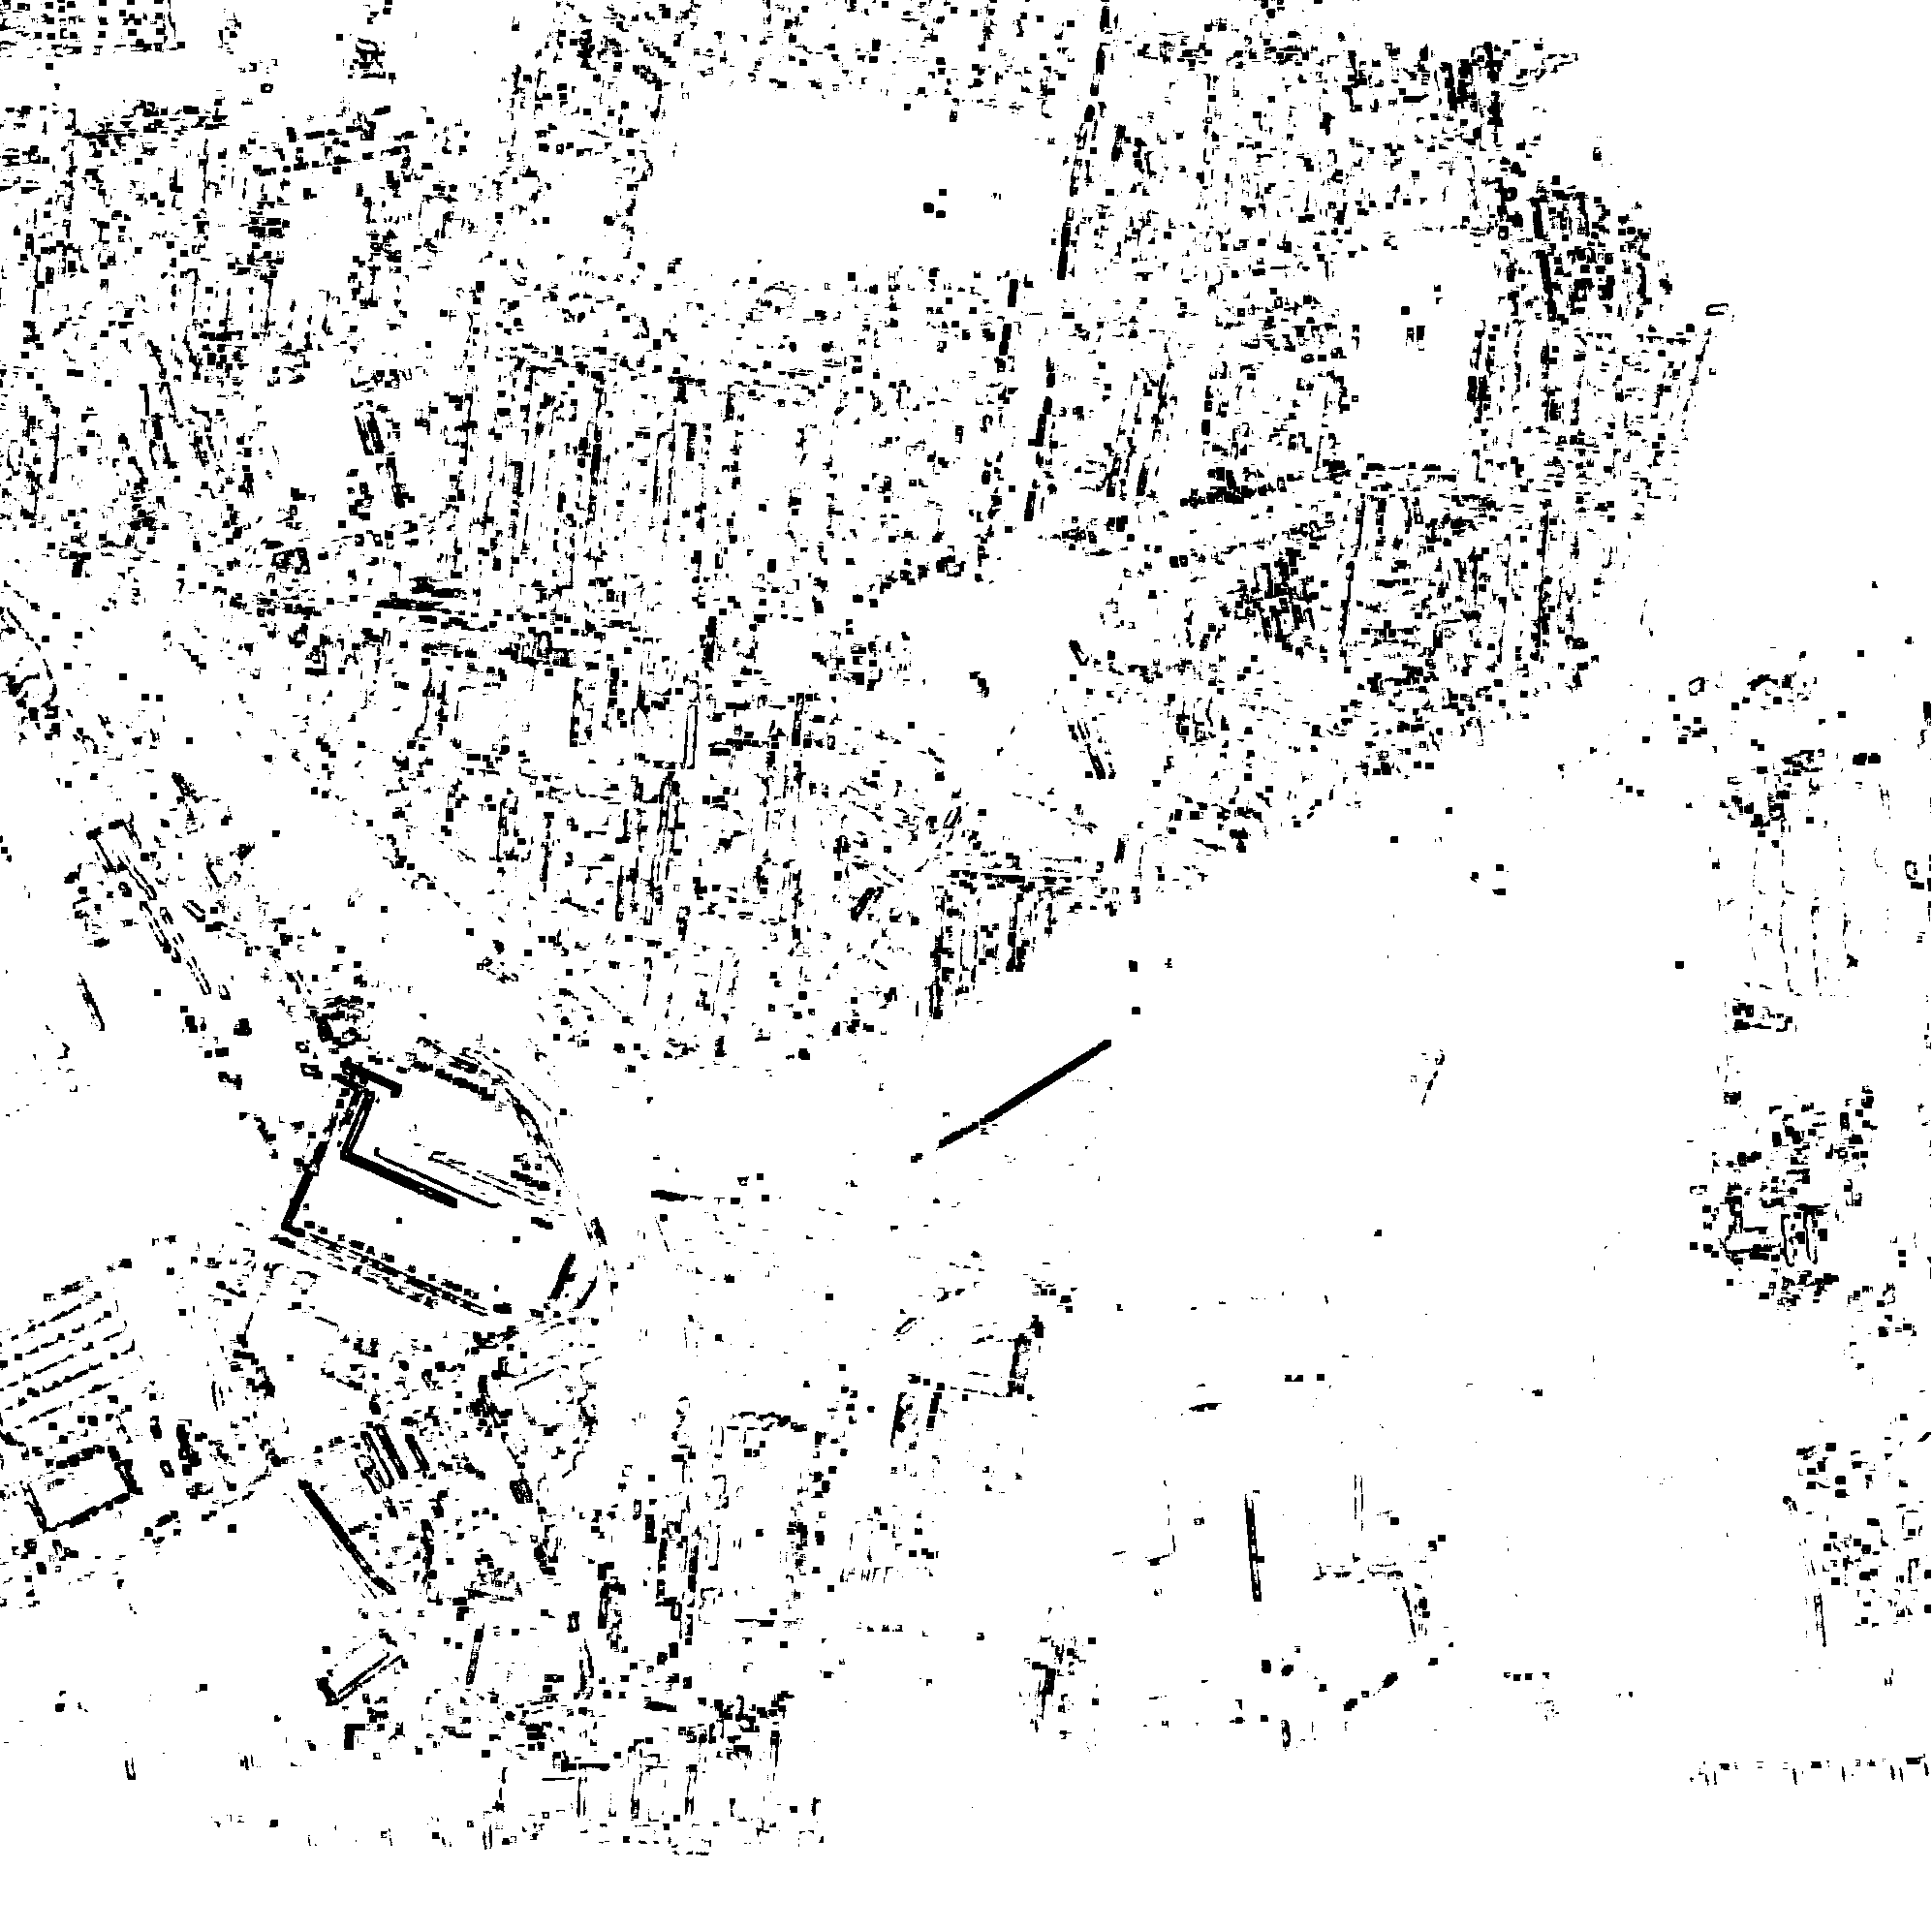
\includegraphics[width=\linewidth]{./Figures/H_005_london_shannon.png}
        \caption{Binary map for $\small{S_{\widetilde{H}_{\text{AO}}}}$}
        \label{fig:1e}
    \end{subfigure}
    \caption{Detection of heterogeneous areas in a SAR image over London, UK: comparison with the tests $\small{S_{\widetilde{H}_{\lambda}}}$ and $\small{S_{\widetilde{H}_{\text{AO}}}}$.  }
    \label{fig:london}
\end{figure*}

\begin{figure*}[hbt]
    \centering
    \begin{subfigure}{0.17\textwidth}
        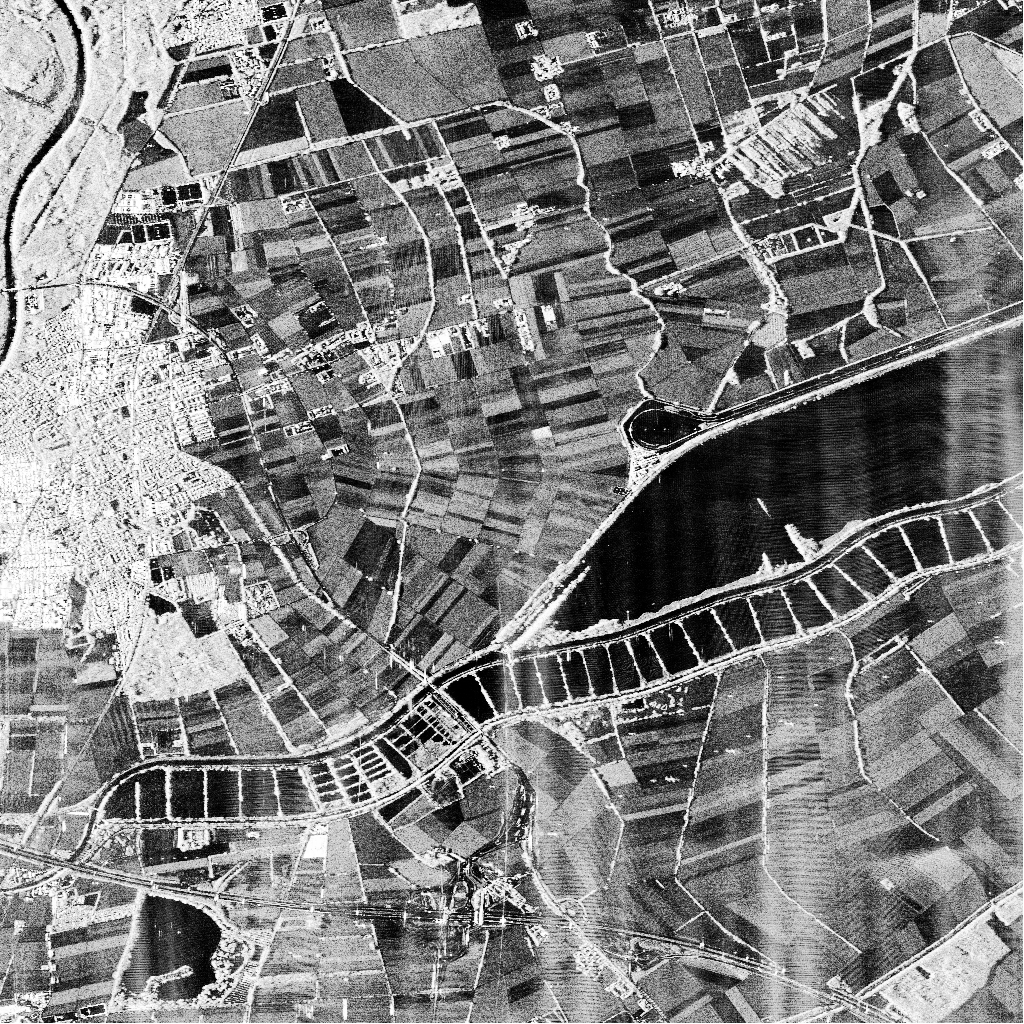
\includegraphics[width=\linewidth]{./Figures/munich_1024_2.png}
        \caption{SAR image}
        \label{fig:2a}
    \end{subfigure}
    \begin{subfigure}{0.23\textwidth}
        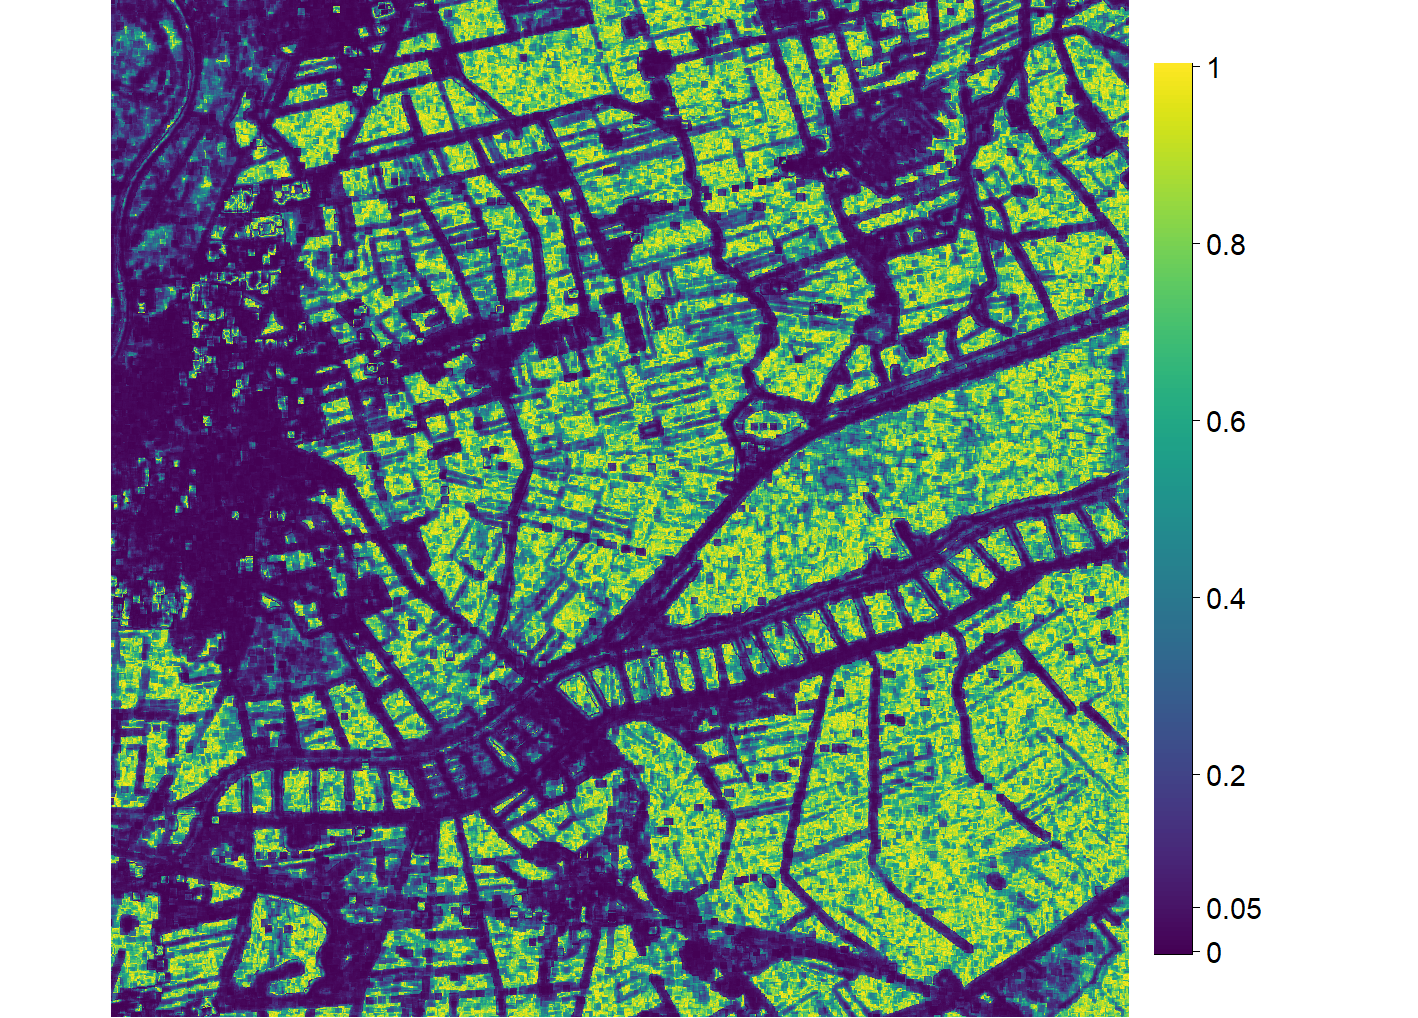
\includegraphics[width=\linewidth]{./Figures/H_pvalue_muni_renyi.png}
        \caption{$p$-values for $\small{S_{\widetilde{H}_{\lambda}}}$}
        \label{fig:2b}
    \end{subfigure}
    \begin{subfigure}{0.16\textwidth}
        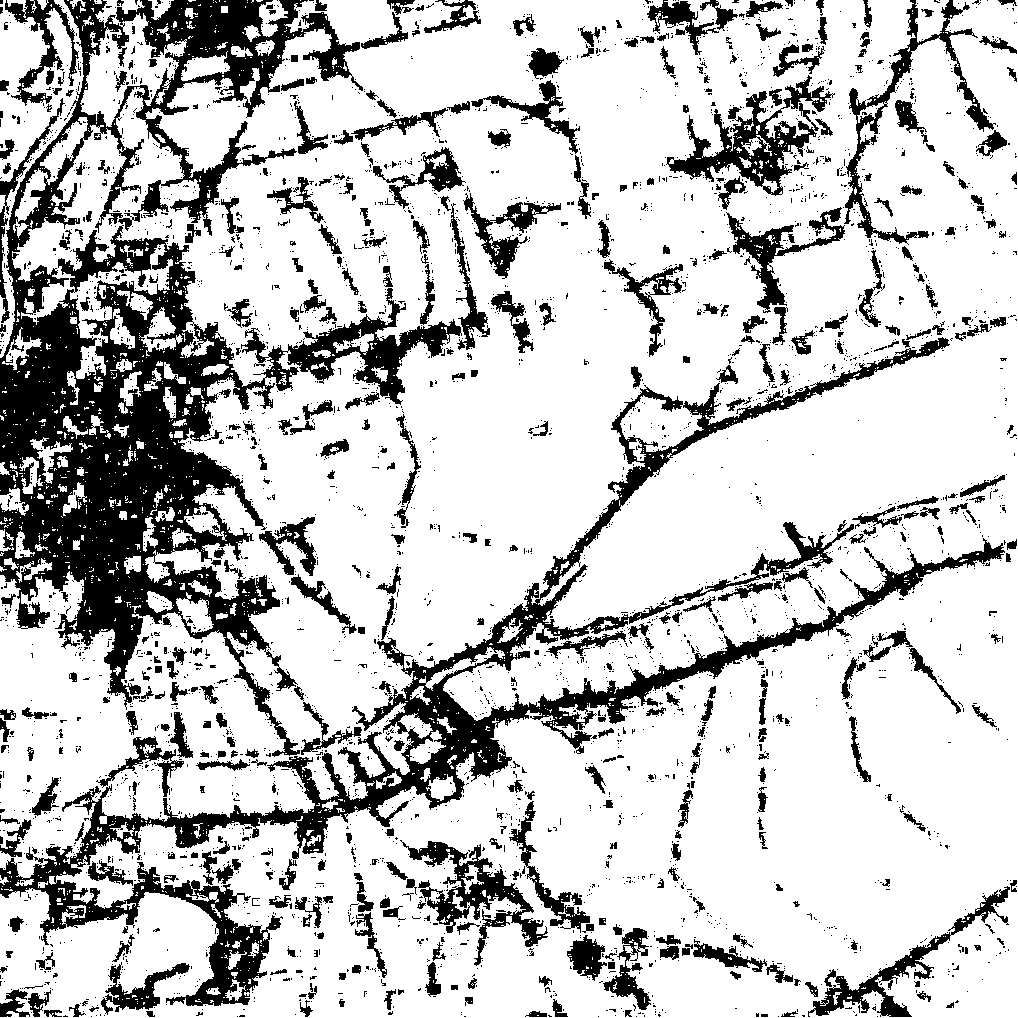
\includegraphics[width=\linewidth]{./Figures/H_005_munich_renyi.png}
        \caption{Binary map for $\small{S_{\widetilde{H}_{\lambda}}}$}
        \label{fig:2c}
    \end{subfigure}
    \begin{subfigure}{0.23\textwidth}
        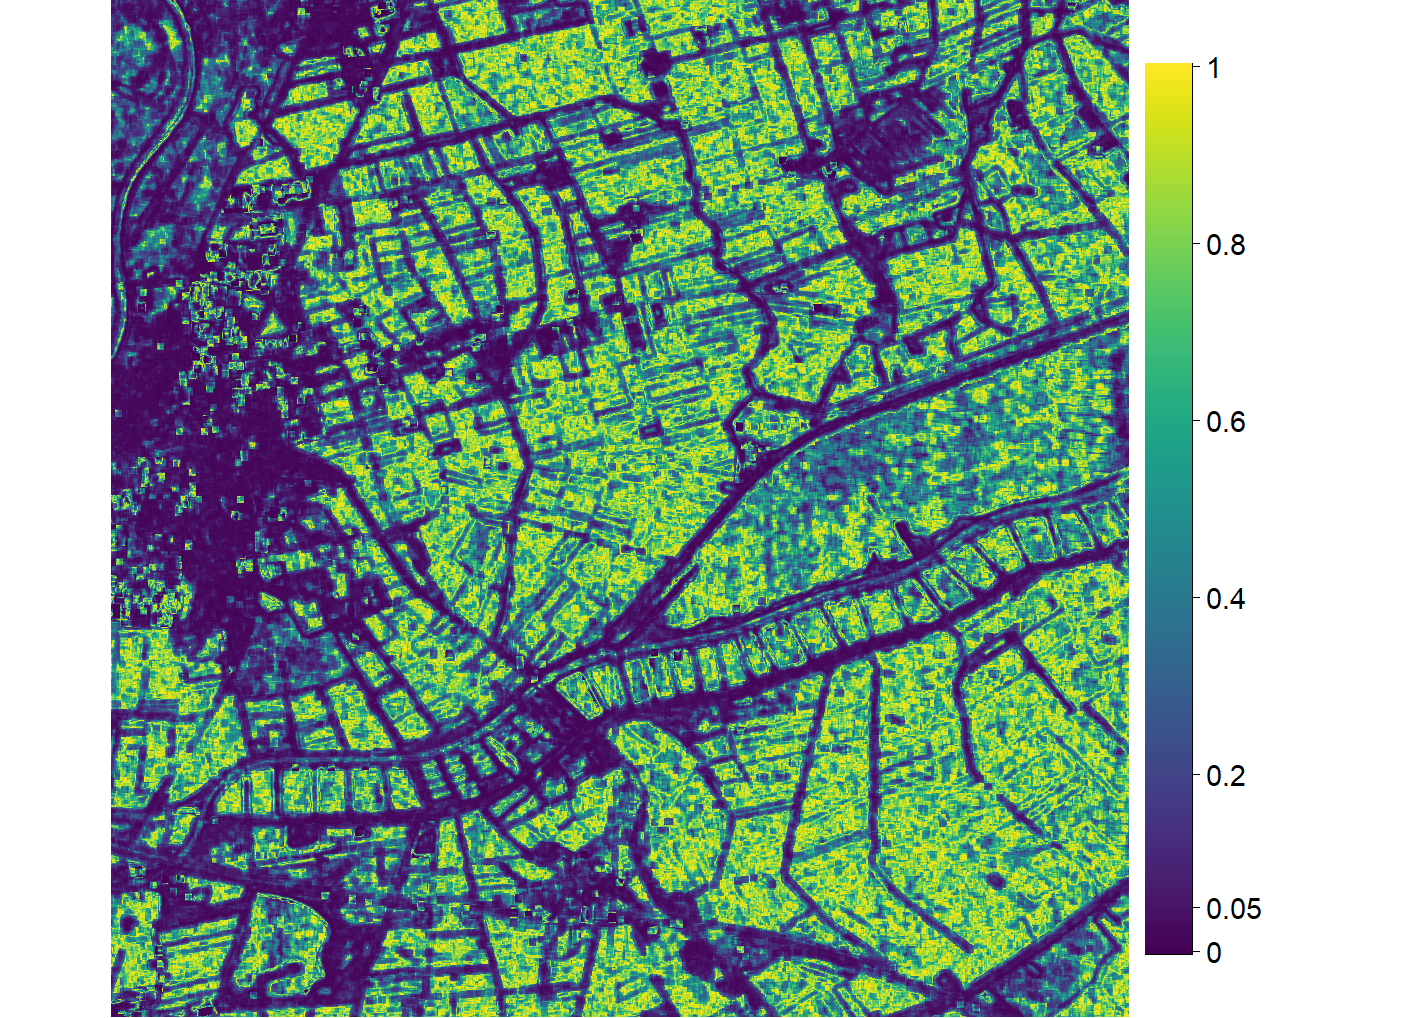
\includegraphics[width=\linewidth]{./Figures/H_pvalue_muni_Shan22.png}
        \caption{$p$-values for $S_{\widetilde{H}_{\text{AO}}}$}
        \label{fig:2d}
    \end{subfigure}
    \begin{subfigure}{0.16\textwidth}
        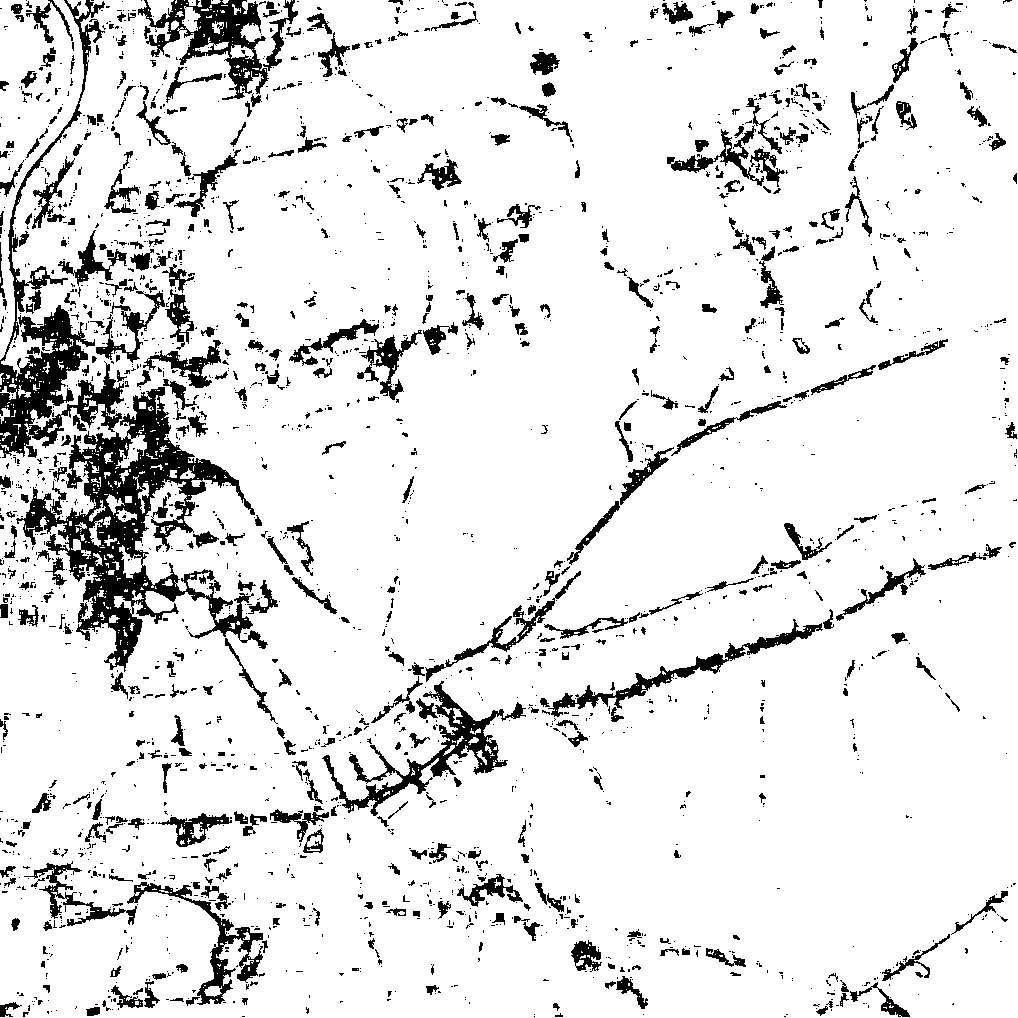
\includegraphics[width=\linewidth]{./Figures/H_005_munich_sh_AO_L12.png}
        \caption{Binary map for $\small{S_{\widetilde{H}_{\text{AO}}}}$}
        \label{fig:2e}
    \end{subfigure}
    \caption{Detection of heterogeneous areas in a SAR image over Munich, Germany: comparison with the tests $\small{S_{\widetilde{H}_{\lambda}}}$ and $\small{S_{\widetilde{H}_{\text{AO}}}}$.}
    \label{fig:munich}
\end{figure*}

\begin{figure*}[hbt]
    \centering
    \begin{subfigure}{0.16\textwidth}
        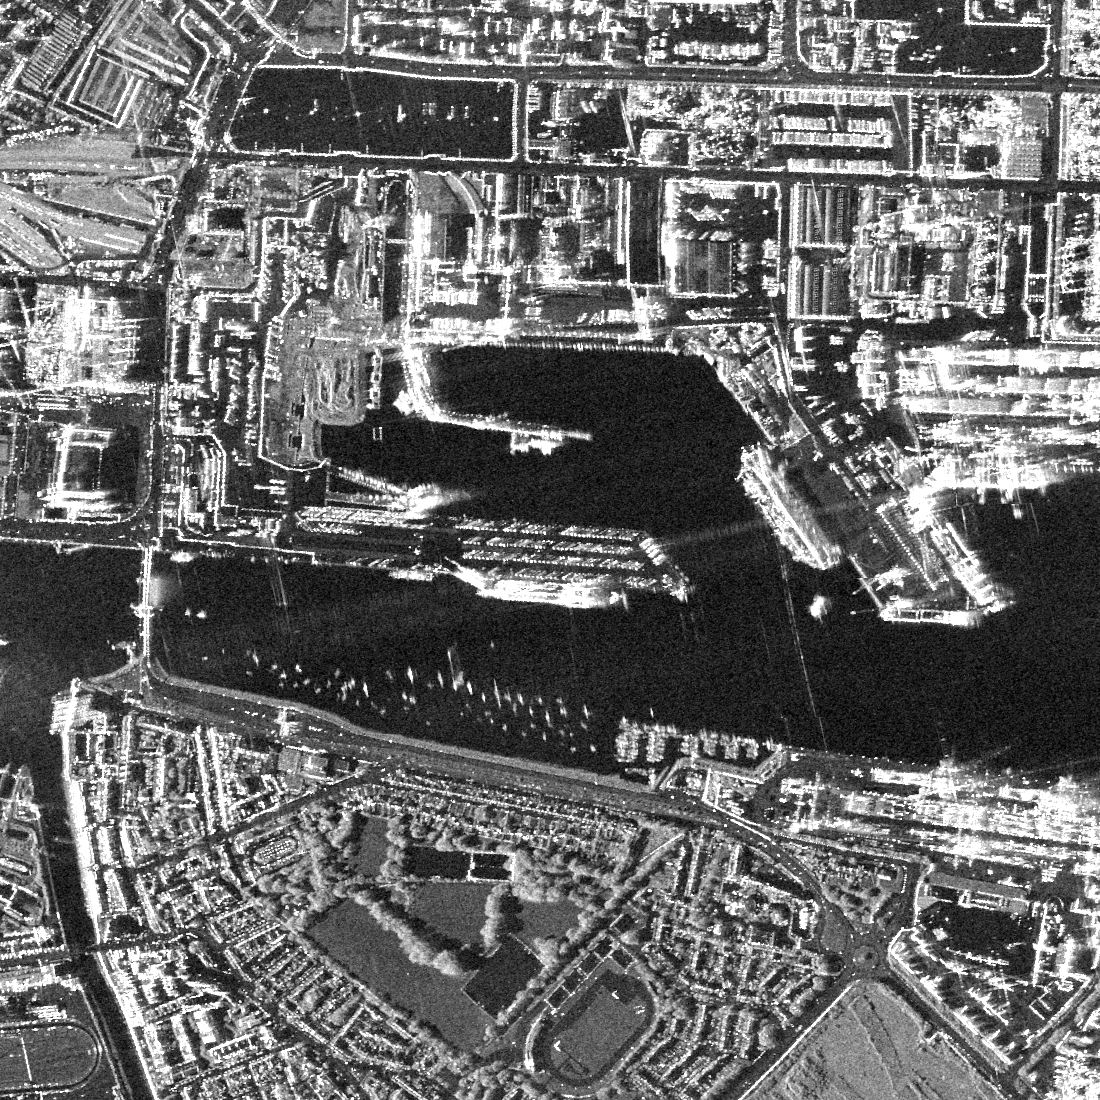
\includegraphics[width=\linewidth]{./Figures/dublin_1100_hh.png}
        \caption{SAR image}
        \label{fig:3a}
    \end{subfigure}
    \begin{subfigure}{0.22\textwidth}
        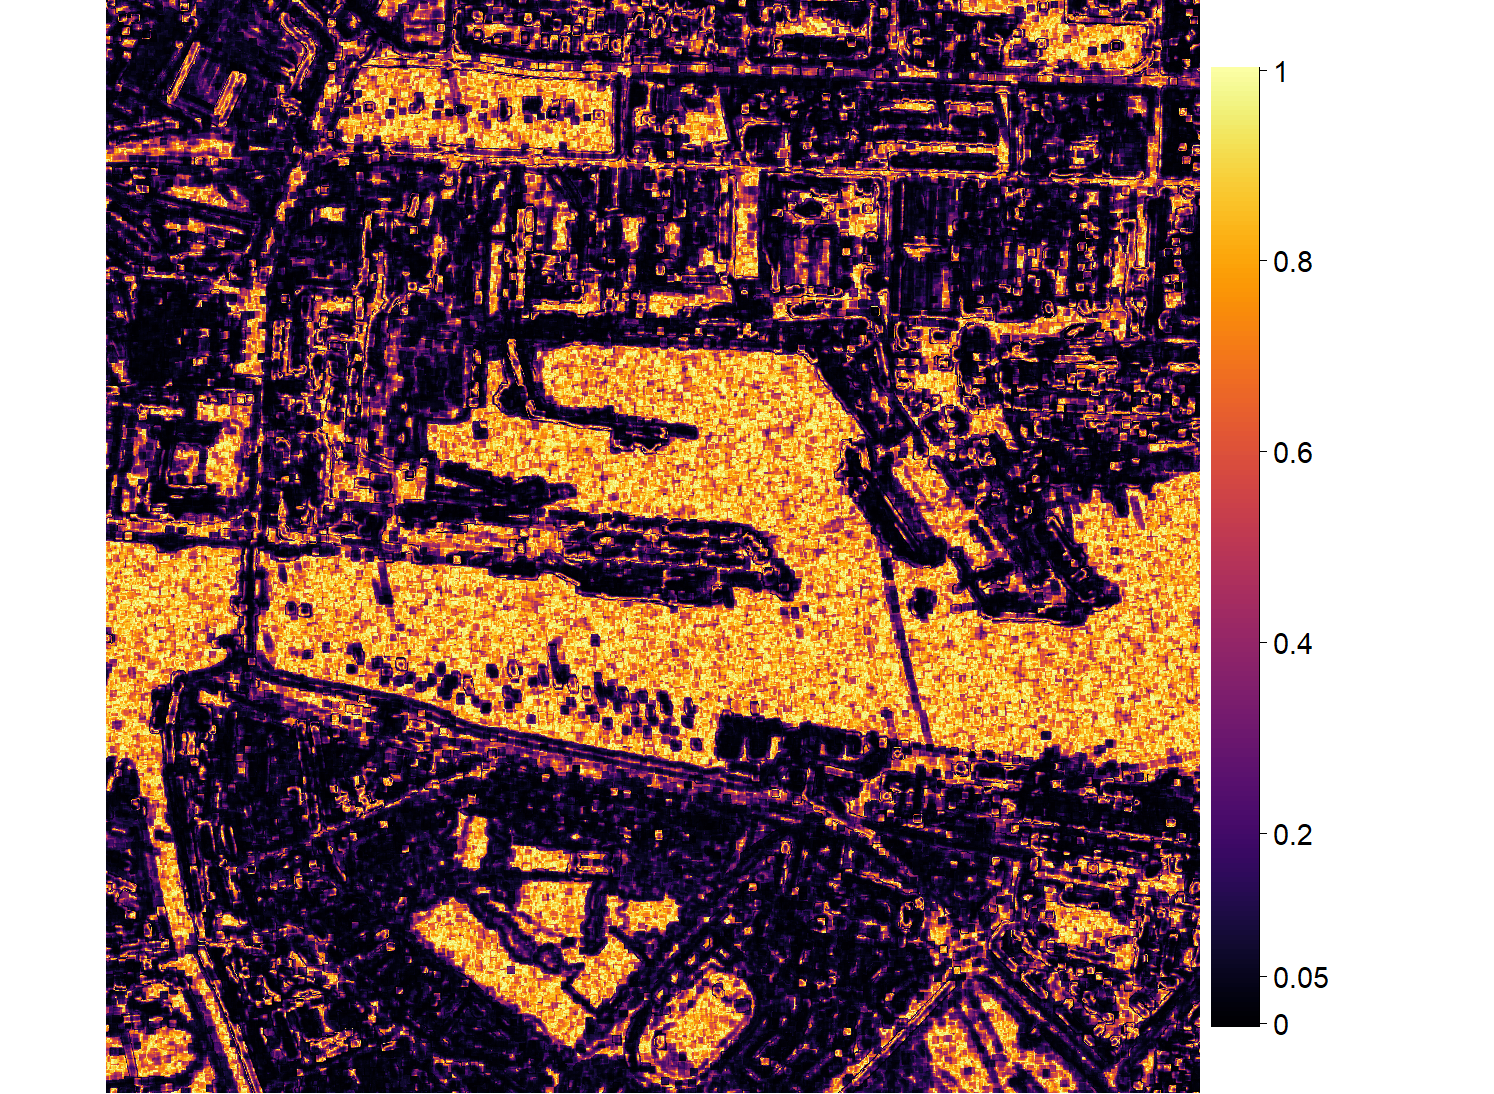
\includegraphics[width=\linewidth]{./Figures/dublin_renyi_09_w7_b100.png}
        \caption{$p$-values for $\small{S_{\widetilde{H}_{\lambda}}}$}
        \label{fig:3b}
    \end{subfigure}
    \begin{subfigure}{0.16\textwidth}
        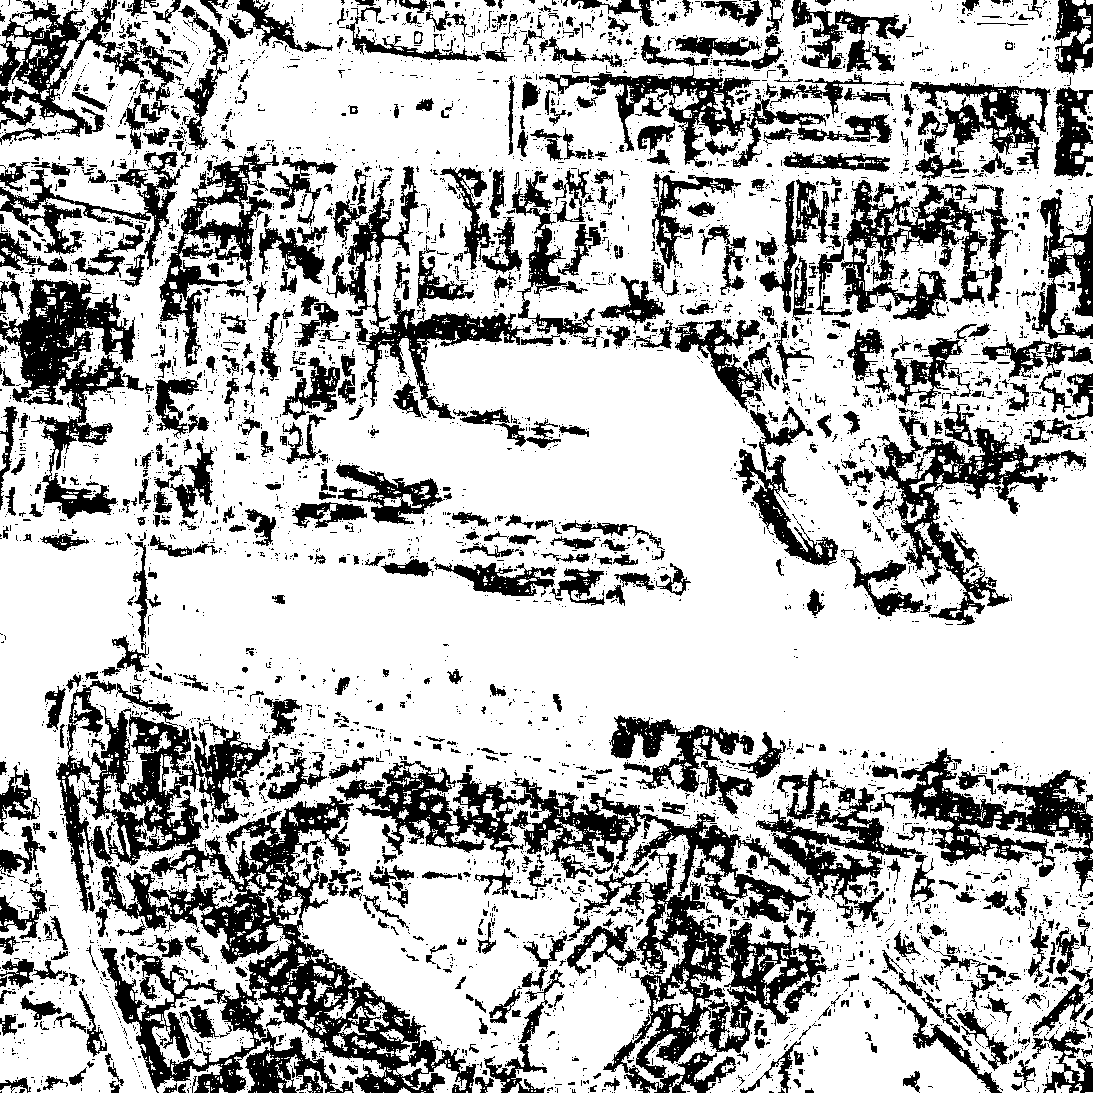
\includegraphics[width=\linewidth]{./Figures/H_005_dublin_renyi_09_w7_b100.png}
        \caption{Binary map for $\small{S_{\widetilde{H}_{\lambda}}}$}
        \label{fig:3c}
    \end{subfigure}
    \begin{subfigure}{0.22\textwidth}
        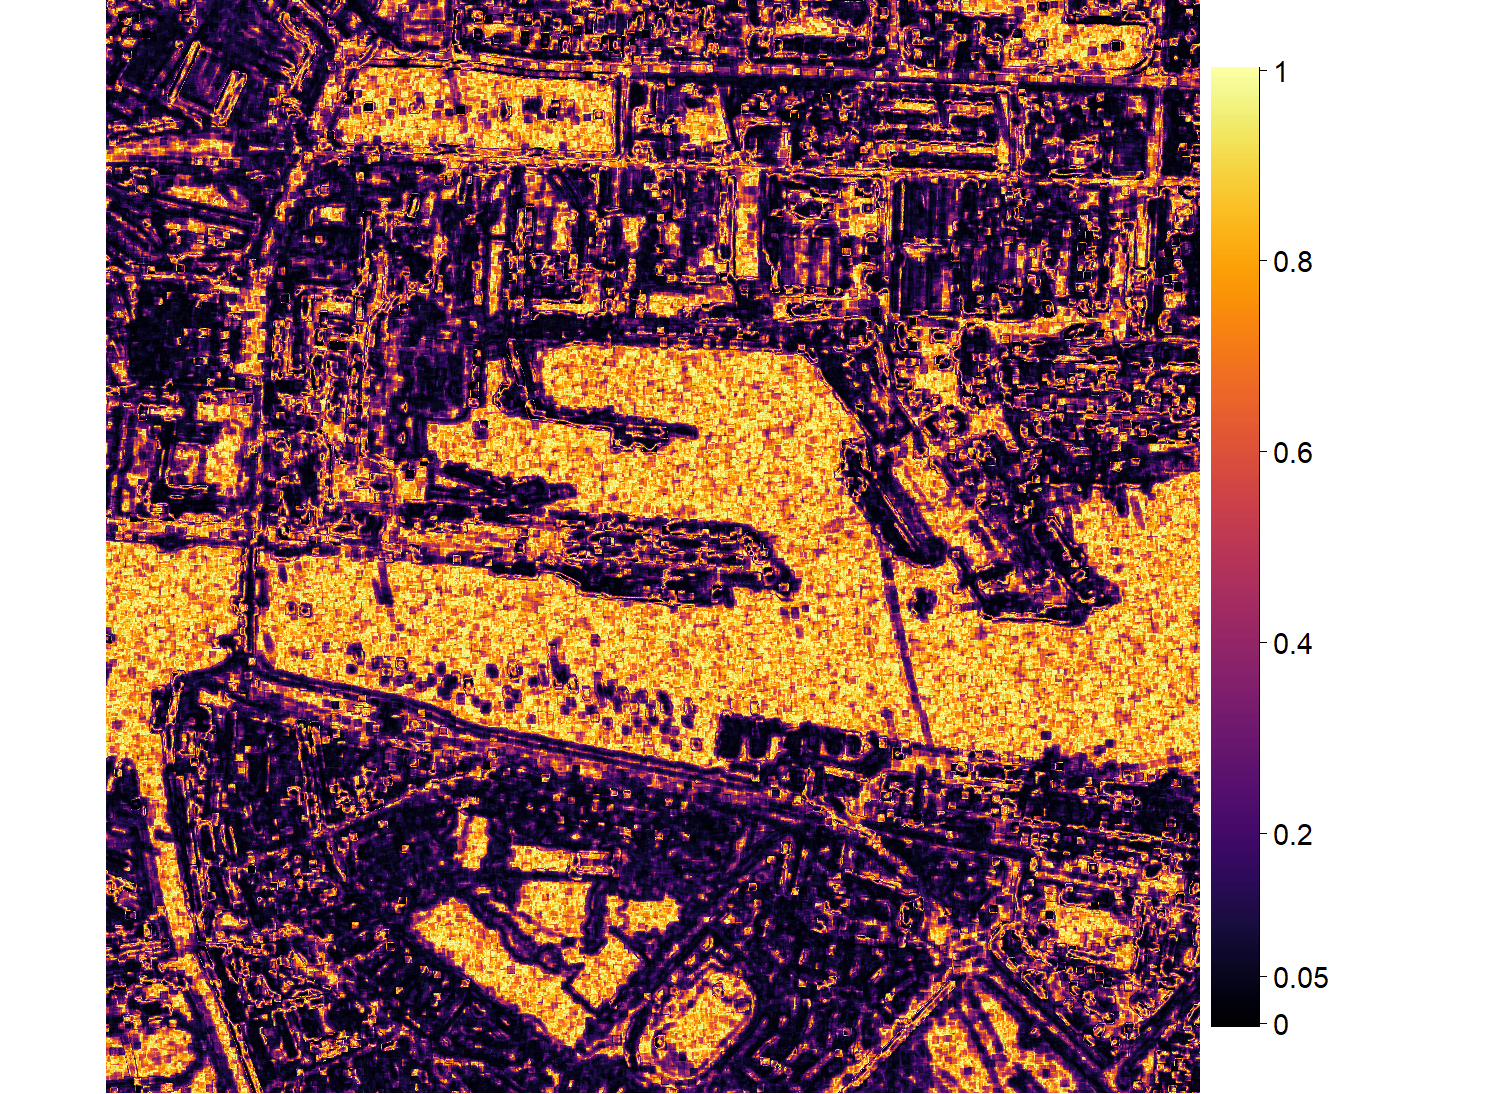
\includegraphics[width=\linewidth]{./Figures/AO_w7_L16_b100.png}
        \caption{$p$-values for $S_{\widetilde{H}_{\text{AO}}}$}
        \label{fig:3d}
    \end{subfigure}
    \begin{subfigure}{0.16\textwidth}
        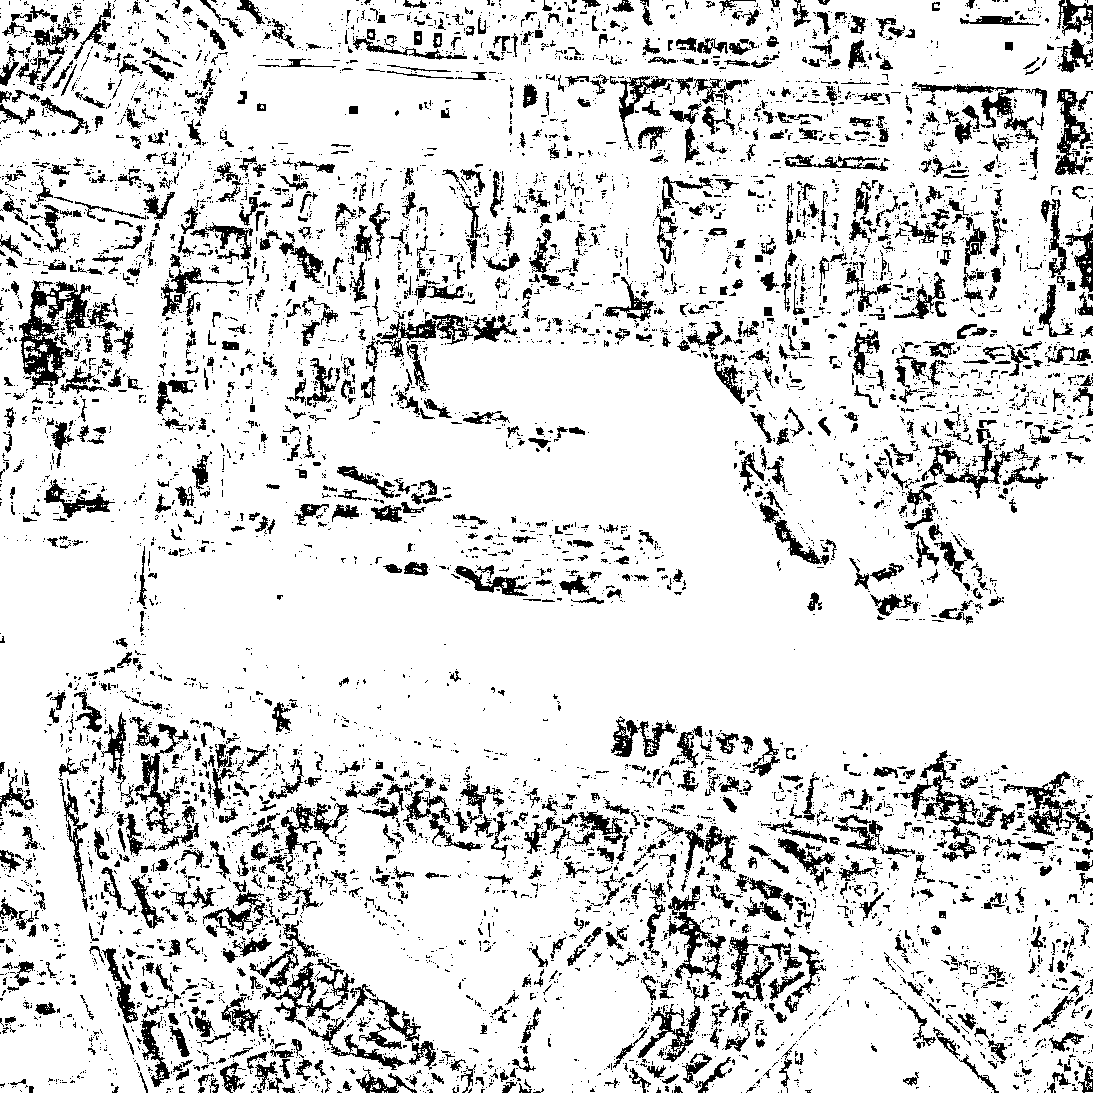
\includegraphics[width=\linewidth]{./Figures/H_005_AO_w7_L16_b100.png}
        \caption{Binary map for $\small{S_{\widetilde{H}_{\text{AO}}}}$}
        \label{fig:3e}
    \end{subfigure}
   \caption{Detection of heterogeneous areas in a SAR image over Dublin Port, Ireland: comparison with the tests $\small{S_{\widetilde{H}_{\lambda}}}$ and $\small{S_{\widetilde{H}_{\text{AO}}}}$.}

    \label{fig:dublin}
\end{figure*}

\section{Conclusion}\label{sec:conclusion}

This study presented a new statistical approach based on Rényi entropy
for detecting heterogeneity in SAR images, distinguishing between fully
developed speckle and heterogeneous clutter. The statistics of the
proposed test was computed nonparametrically and its performance was
evaluated by a Monte Carlo study. The results showed that the method
effectively controls the probability of type I error while maintaining a
high detection performance that improves as the sample size increases.

The performance of the Rényi-based test was evaluated by comparing its
results with those of a test based on Shannon entropy. This comparison
was performed using \(p\)-values and binary maps. The results showed
that while both tests successfully detected heterogeneous regions, the
Rényi-based test performed better due to its flexibility in adjusting
the \(\lambda\) parameter, which allowed for finer differentiation of
texture variations.

These results suggested that the Rényi entropy was a more accurate
alternative to the Shannon entropy for detecting heterogeneity in SAR
images, especially due to its adaptability.

Future research will focus on a more quantitative evaluation of both
approaches, using statistical measures such as mean square error and
other validation metrics to assess their accuracy in detecting
heterogeneity.

\appendix[Derivation of the Rényi Entropy of $\mathcal{G}^0_I$]{}

Let \(Z \sim \mathcal{G}^0_I(\alpha, \gamma, L)\), defined
in~\citeproc{ref-Frery2024}{{[}12{]}}, we compute
\(I = \int_0^\infty [f_{\mathcal{G}^0_I}(z)]^\lambda dz\). Using the
pdf\\
\begin{equation*}
f_{\mathcal{G}^0_I}(z) = C \frac{z^{L-1}}{(\gamma + Lz)^{L-\alpha}},  
\quad C = \frac{L^L \Gamma(L - \alpha)}{\gamma^\alpha \Gamma(-\alpha) \Gamma(L)}, \label{eq:pdf_G0I}
\end{equation*} and setting \(t = Lz/\gamma\), we obtain\\
\begin{equation*}
I = C^\lambda \frac{\gamma^{1-\lambda+\lambda\alpha}}{L^{\lambda L + 1 - \lambda}}  
\int_0^\infty \frac{t^{\lambda(L-1)}}{(1+t)^{\lambda(L-\alpha)}} dt.
\end{equation*} Applying the Beta function identity,
\(B(a,b) = \int_0^\infty \frac{t^{a-1}}{(1+t)^{a+b}} dt\) with
\(a = \lambda(L-1) + 1\), \(b = \lambda(-\alpha+1) - 1\), we get\\
\begin{equation*}
I= \gamma^{\,1 - \lambda}\,
   L^{\,\lambda - 1}
   \Bigl(\tfrac{\Gamma(L - \alpha)}{\Gamma(-\alpha)\,\Gamma(L)}\Bigr)^\lambda
   \,B(a,b).
\end{equation*} Using the Rényi entropy definition in
\eqref{E:entropy2}: \(H_\lambda(Z) = \frac{1}{1-\lambda} \ln I\), and
substituting \(\gamma = -\mu(\alpha + 1)\), we obtain the final
expression for \(\mathcal{G}^0_I(\mu, \alpha, L)\) in \eqref{eq-HGI0}.

Code is available at: \url{https://github.com/rjaneth/renyi-entropy}

\section*{References}\label{references}
\addcontentsline{toc}{section}{References}

\phantomsection\label{refs}
\begin{CSLReferences}{0}{0}
\bibitem[\citeproctext]{ref-Yu2023}
\CSLLeftMargin{{[}1{]} }%
\CSLRightInline{H. Yu, X. Yin, Z. Liu, S. Zhou, C. Li, and H. Jiang,
{``\href{https://doi.org/10.1109/jstars.2023.3257548}{A novel
unsupervised evaluation metric based on heterogeneity features for SAR
image segmentation},''} \emph{IEEE Journal of Selected Topics in Applied
Earth Observations and Remote Sensing}, vol. 16, pp. 2851--2867, 2023. }

\bibitem[\citeproctext]{ref-Akbarizadeh2012}
\CSLLeftMargin{{[}2{]} }%
\CSLRightInline{G. Akbarizadeh,
{``\href{https://doi.org/10.1109/tgrs.2012.2194787}{A new
statistical-based kurtosis wavelet energy feature for texture
recognition of SAR images},''} \emph{IEEE Transactions on Geoscience and
Remote Sensing}, vol. 50, no. 11, pp. 4358--4368, 2012. }

\bibitem[\citeproctext]{ref-Mondini2021}
\CSLLeftMargin{{[}3{]} }%
\CSLRightInline{A. C. Mondini, F. Guzzetti, K.-T. Chang, O. Monserrat,
T. R. Martha, and A. Manconi,
{``\href{https://doi.org/10.1016/j.earscirev.2021.103574}{Landslide
failures detection and mapping using synthetic aperture radar: Past,
present and future},''} \emph{Earth-Science Reviews}, vol. 216, p.
103574, 2021. }

\bibitem[\citeproctext]{ref-Zeng2020}
\CSLLeftMargin{{[}4{]} }%
\CSLRightInline{Z. Zeng \emph{et al.},
{``\href{https://doi.org/10.1016/j.jhydrol.2019.124377}{Towards high
resolution flood monitoring: An integrated methodology using passive
microwave brightness temperatures and sentinel synthetic aperture radar
imagery},''} \emph{Journal of Hydrology}, vol. 582, p. 124377, 2020. }

\bibitem[\citeproctext]{ref-Argenti2013}
\CSLLeftMargin{{[}5{]} }%
\CSLRightInline{F. Argenti, A. Lapini, T. Bianchi, and L. Alparone,
{``\href{https://doi.org/10.1109/mgrs.2013.2277512}{A tutorial on
speckle reduction in synthetic aperture radar images},''} \emph{IEEE
Geoscience and Remote Sensing Magazine}, vol. 1, no. 3, pp. 6--35, 2013.
}

\bibitem[\citeproctext]{ref-Choi2019}
\CSLLeftMargin{{[}6{]} }%
\CSLRightInline{H. Choi and J. Jeong,
{``\href{https://doi.org/10.3390/rs11101184}{Speckle noise reduction
technique for SAR images using statistical characteristics of speckle
noise and discrete wavelet transform},''} \emph{Remote Sensing}, vol.
11, no. 10, p. 1184, 2019. }

\bibitem[\citeproctext]{ref-Nascimento2014}
\CSLLeftMargin{{[}7{]} }%
\CSLRightInline{A. D. C. Nascimento, M. M. Horta, A. C. Frery, and R. J.
Cintra, {``Comparing edge detection methods based on stochastic
entropies and distances for {PolSAR} imagery,''} \emph{{IEEE} Journal of
Selected Topics in Applied Earth Observations and Remote Sensing}, vol.
7, no. 2, pp. 648--663, 2014. }

\bibitem[\citeproctext]{ref-Nobre2016}
\CSLLeftMargin{{[}8{]} }%
\CSLRightInline{R. H. Nobre, F. A. A. Rodrigues, R. C. P. Marques, J. S.
Nobre, J. F. S. R. Neto, and F. N. S. Medeiros,
{``\href{https://doi.org/10.1109/lsp.2016.2606760}{SAR image
segmentation with {R}ényi's entropy},''} \emph{IEEE Signal Processing
Letters}, vol. 23, no. 11, pp. 1551--1555, 2016. }

\bibitem[\citeproctext]{ref-Cassetti2022}
\CSLLeftMargin{{[}9{]} }%
\CSLRightInline{J. Cassetti, D. Delgadino, A. Rey, and A. C. Frery,
{``Entropy estimators in {SAR} image classification,''} \emph{Entropy},
vol. 24, no. 4, p. 509, 2022. }

\bibitem[\citeproctext]{ref-Chan2022}
\CSLLeftMargin{{[}10{]} }%
\CSLRightInline{D. Chan, J. Gambini, and A. C. Frery,
{``\href{https://doi.org/10.3390/rs14030509}{Entropy-based non-local
means filter for single-look SAR speckle reduction},''} \emph{Remote
Sensing}, vol. 14, no. 3, p. 509, 2022. }

\bibitem[\citeproctext]{ref-Shannon1948}
\CSLLeftMargin{{[}11{]} }%
\CSLRightInline{C. E. Shannon, {``A mathematical theory of
communication,''} \emph{The Bell System Technical Journal}, vol. 27, no.
3, pp. 379--423, 1948. }

\bibitem[\citeproctext]{ref-Frery2024}
\CSLLeftMargin{{[}12{]} }%
\CSLRightInline{A. C. Frery, J. Alpala, and A. D. C. Nascimento,
{``\href{https://doi.org/10.3390/rs16111973}{Identifying heterogeneity
in SAR data with new test statistics},''} \emph{Remote Sensing}, vol.
16, no. 11, p. 1973, 2024. }

\bibitem[\citeproctext]{ref-Frery1997}
\CSLLeftMargin{{[}13{]} }%
\CSLRightInline{A. C. Frery, H.-J. Muller, C. C. F. Yanasse, and S. J.
S. SantAnna, {``A model for extremely heterogeneous clutter,''}
\emph{{IEEE} Transactions on Geoscience and Remote Sensing}, vol. 35,
no. 3, pp. 648--659, 1997. }

\bibitem[\citeproctext]{ref-renyi1961measures}
\CSLLeftMargin{{[}14{]} }%
\CSLRightInline{A. Rényi, {``On measures of entropy and information,''}
in \emph{Proceedings of the fourth berkeley symposium on mathematical
statistics and probability, volume 1: Contributions to the theory of
statistics}, 1961, vol. 4, pp. 547--562. }

\bibitem[\citeproctext]{ref-Ribeiro2021}
\CSLLeftMargin{{[}15{]} }%
\CSLRightInline{M. Ribeiro \emph{et al.},
{``\href{https://doi.org/10.3390/e23020222}{The entropy universe},''}
\emph{Entropy}, vol. 23, no. 2, p. 222, 2021. }

\bibitem[\citeproctext]{ref-vasicek1976test}
\CSLLeftMargin{{[}16{]} }%
\CSLRightInline{O. Vasicek, {``A test for normality based on sample
entropy,''} \emph{Journal of the Royal Statistical Society Series B:
Statistical Methodology}, vol. 38, no. 1, pp. 54--59, 1976. }

\bibitem[\citeproctext]{ref-Ebrahimi1994}
\CSLLeftMargin{{[}17{]} }%
\CSLRightInline{N. Ebrahimi, K. Pflughoeft, and E. S. Soofi, {``Two
measures of sample entropy,''} \emph{Statistics \& Probability Letters},
vol. 20, no. 3, pp. 225--234, 1994. }

\bibitem[\citeproctext]{ref-Wieczorkowski1999}
\CSLLeftMargin{{[}18{]} }%
\CSLRightInline{R. Wieczorkowski and P. Grzegorzewski, {``Entropy
estimators-improvements and comparisons,''} \emph{Communications in
Statistics-Simulation and Computation}, vol. 28, no. 2, pp. 541--567,
1999. }

\bibitem[\citeproctext]{ref-AlOmari2019}
\CSLLeftMargin{{[}19{]} }%
\CSLRightInline{A. I. Al-Omari and A. Haq, {``Novel entropy estimators
of a continuous random variable,''} \emph{International Journal of
Modeling, Simulation, and Scientific Computing}, vol. 10, no. 2, p.
1950004, 2019. }

\bibitem[\citeproctext]{ref-AlLabadi2024}
\CSLLeftMargin{{[}20{]} }%
\CSLRightInline{L. Al-Labadi, Z. Chu, and Y. Xu,
{``\href{https://doi.org/10.1007/s00180-024-01507-z}{Advancements in
{R}ényi entropy and divergence estimation for model assessment},''}
\emph{Computational Statistics}, 2024. }

\bibitem[\citeproctext]{ref-Alpala2024}
\CSLLeftMargin{{[}21{]} }%
\CSLRightInline{R. J. Alpala, A. D. C. Nascimento, and A. C. Frery,
{``\href{https://doi.org/10.1109/migars61408.2024.10544448}{Identifying
departures from the fully developed speckle hypothesis in intensity SAR
data with non-parametric estimation of the entropy},''} in \emph{2024
international conference on machine intelligence for GeoAnalytics and
remote sensing (MIGARS)}, 2024, pp. 1--4. }

\end{CSLReferences}


% Can use something like this to put references on a page
% by themselves when using endfloat and the captionsoff option.
\ifCLASSOPTIONcaptionsoff
  \newpage
\fi

% trigger a \newpage just before the given reference
% number - used to balance the columns on the last page
% adjust value as needed - may need to be readjusted if
% the document is modified later
%\IEEEtriggeratref{8}
% The "triggered" command can be changed if desired:
%\IEEEtriggercmd{\enlargethispage{-5in}}

% Uncomment when use biblatex with style=ieee
%\renewcommand{\bibfont}{\footnotesize} % for IEEE bibfont size

\pagebreak[3]
% that's all folks
\end{document}

